\documentclass{myclass}
\usepackage[polish]{babel}

\author{Bartosz Hanc}
\title{Uczenie głębokie --- zarys}

\begin{document}

\maketitle

\section{Wprowadzenie}

Historia sztucznych sieci neuronowych sięga lat 50. XX wieku, kiedy to Frank Rosenblatt zaproponował
model perceptronu -- prostej 3-warstwowej sieci, której zadaniem miało być rozpoznawanie znaków
alfanumerycznych. Podstawową jednostką przetwarzającą w takiej sieci był neuron McCullocha--Pittsa,
który realizował następujące przekształcenie \(F: \Rbb^n \mapsto \Rbb\)
\[
    F(\bm{x}) = \varphi \left( \bm{x} \bm{w}^\tpose + b \right)\,,
\]
gdzie \(\bm{x} = (x_1, \ldots, x_n)\) określa sygnały wchodzące do neuronu, \(\varphi\) jest pewną
nieliniową funkcję zwaną funkcją aktywacji, a \(\bm{w}\) i \(b\) to pewne parametry (zwane również
wagami) określające, które z sygnałów mają być wzmocnione, a które osłabione. Perceptron jest
zbudowany z wielu takich neuronów połączonych ze sobą. Neurony te są zorganizowane w warstwy, w
obrębie których nie ma połączeń, natomiast między sąsiednimi warstwami neurony są połączone ,,każdy
z każdym''. Na Rysunku \ref{fig:nn} przedstawiono schemat takiego prostego perceptronu
wielowarstwowego. Strzałki pokazują przepływ sygnałów w sieci, natomiast każdy wierzchołek
reprezentuje odwzorowanie nieliniowe \(F\) z właściwymi dla siebie wagami. Efektywnie perceptron
wielowarstwowy realizuje więc pewne przekształcenie nieliniowe \(\Rbb^n \mapsto \Rbb^m\).

\begin{figure}[ht]
    \centering
    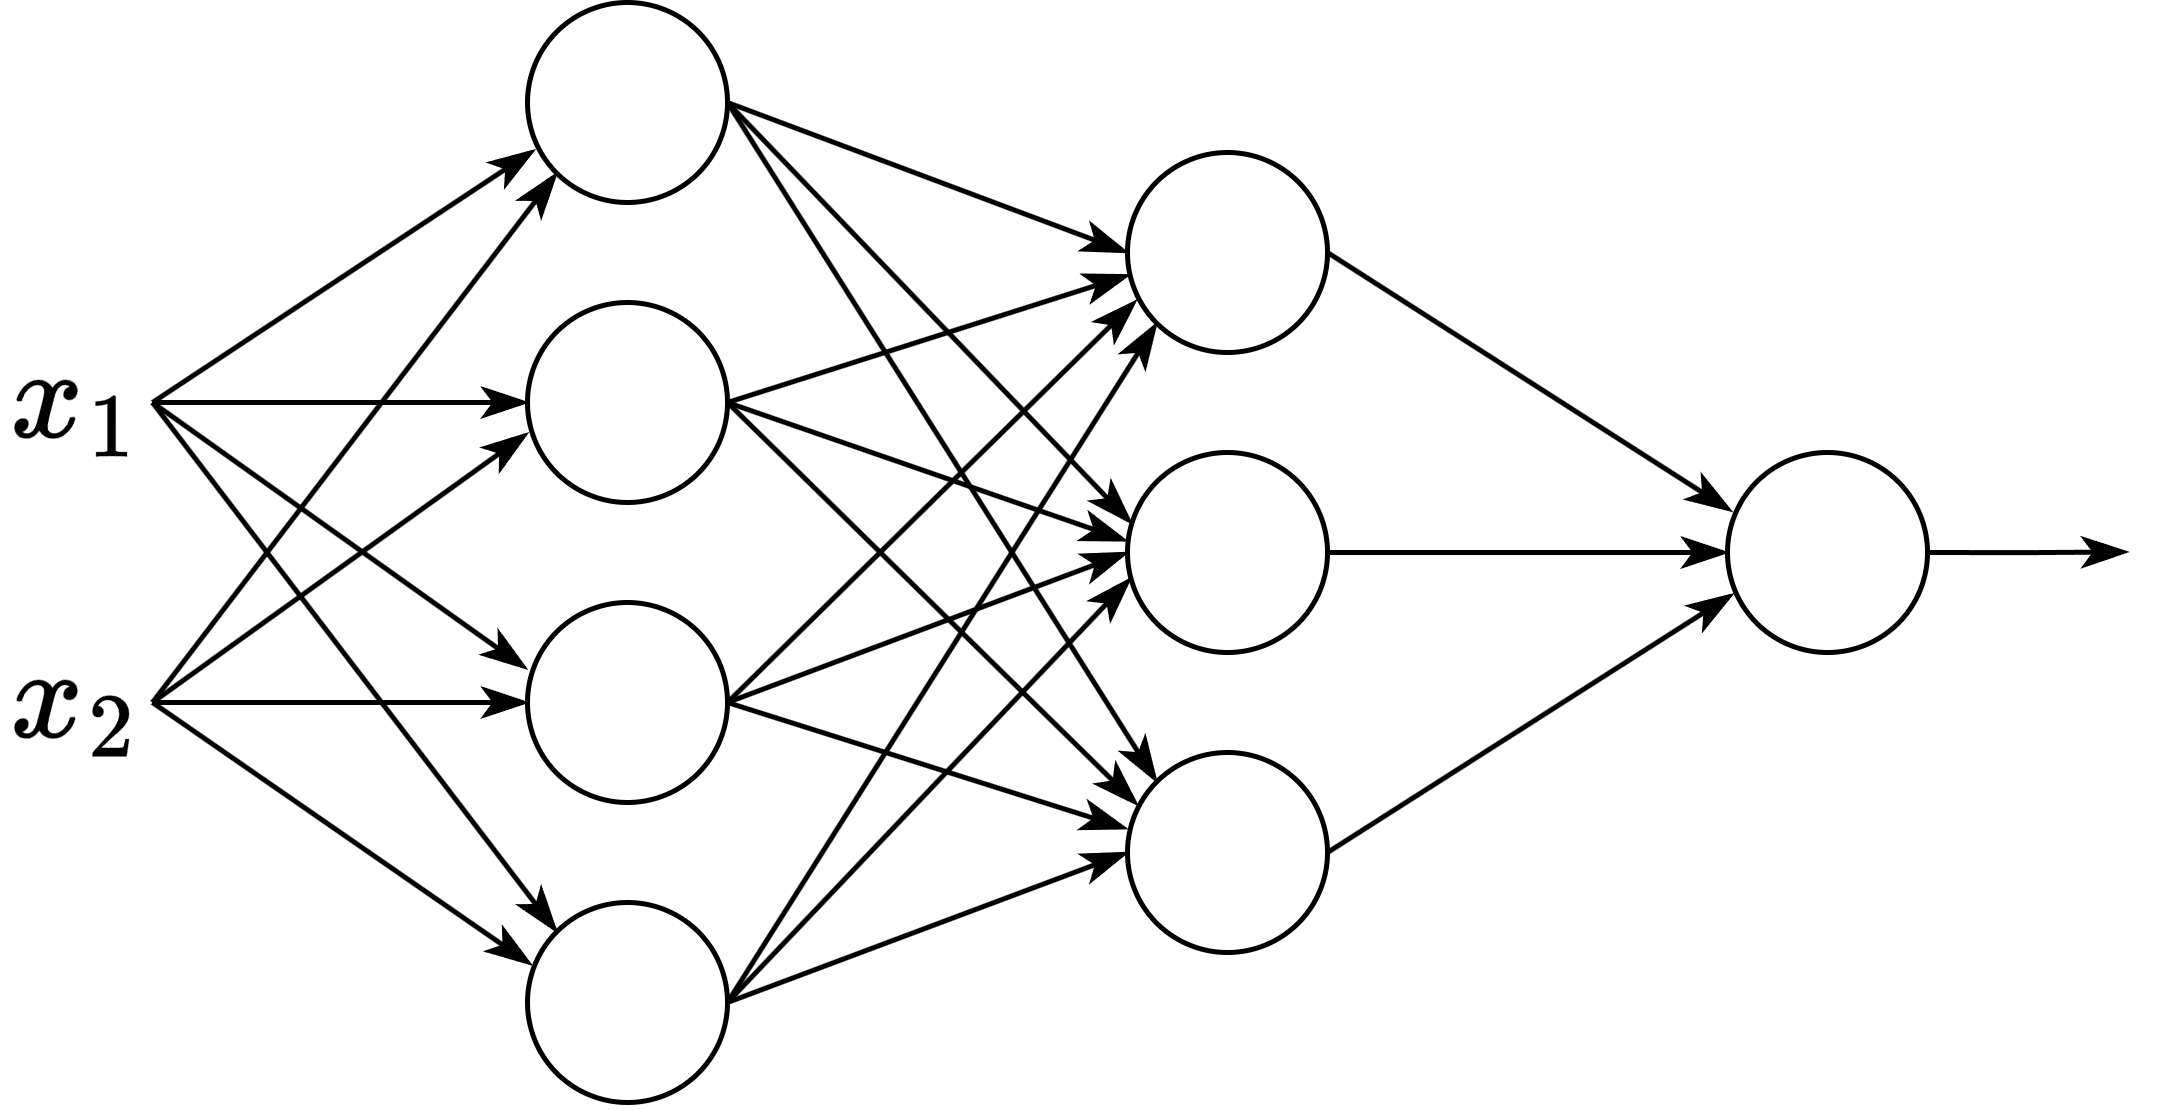
\includegraphics[width=0.85\linewidth]{figs/nn.png}
    \label{fig:nn}
    \caption{Schemat prostego perceptronu wielowarstwowego realizującego odwzorowanie \(\Rbb^2 \mapsto \Rbb\)}
\end{figure}

Podany powyżej opis konstrukcji sztucznych sieci neuronowych, choć często przywoływany we
wprowadzeniach, nie jest zbyt użyteczny w nowoczesnym podejściu do uczenia głębokiego. Bardziej
przydatnym sformułowaniem, czym właściwie są sieci neuronowe jest następująca definicja: sieć
neuronowa to dowolny skierowany graf acykliczny, którego wierzchołki reprezentują dowolną
sparametryzowaną funkcję o argumentach i wartościach tensorowych, a skierowane krawędzie
reprezentują przepływ tych tensorów. Sieć neuronowa realizuje więc pewne przekształcenie wejściowych
tensorów (przykładowo może to być 4-wymiarowy tensor reprezentujący zbiór kolorowych obrazków).
Trening sieci neuronowej będzie polegał na takiej zmianie jej parametrów, aby sieć realizowała
określone zadanie.

\medskip

Pojęcie tensora w uczeniu maszynowym nie ma wiele wspólnego z tensorami używanymi w algebrze, czy w
fizyce. W naszym kontekście tensor to po prostu wielowymiarowa tablica liczb. Standardowo w tym
tekście tensory będziemy oznaczać literami wytłuszczonymi, np. \(\bm{A}\), natomiast odnosząc się do
ustalonego elementu tensora \(\bm{A}\) będziemy zapisywać \(A_{\alpha_1,\ldots,\alpha_k}\) lub
\(A_\alpha\), gdzie \(\alpha\) będzie oznaczać wielowskaźnik \((\alpha_1,\ldots,\alpha_k)\). Liczbę
\(k\) nazywamy wymiarem tensora \(\bm{A}\). Zbiór wszystkich tensorów wymiaru \(k\) o liczbie
elementów wzdłuż osi \(i\) równej \(n_i\) będziemy oznaczać \(\Rbb^{(n_1,\ldots,n_k)}\).

\medskip

Mamy więc graf skierowany posiadający \(N\) wierzchołków. Dla każdego wierzchołka \(i \in [N]\)
wprowadzimy następujące wielkości:
\begin{itemize}
    \item \(\mathscr{N}_i\) -- zbiór następników, tj. wierzchołków \(j \in [N]\), dla których
    istnieje krawędź skierowana \((i,j)\),
    
    \item \(\mathscr{P}_i\) -- zbiór poprzedników, tj. wierzchołków \(j \in [N]\), dla których
    istnieje krawędź skierowana \((j,i)\),

    \item \(\bm{F}^{(i)}\left(\cdot ; \bm{\theta}^{(i)}\right)\) -- funkcję tensorową realizowaną
    przez dany wierzchołek, sparametryzowaną przez \(\bm{\theta}^{(i)}\),

    \item \(\bm{v}^{(i)}\) -- wartość funkcji \(\bm{F}^{(i)}\) przechowywaną aktualnie w wierzchołku
    (w szczególności może to być tzw. null -- \(\varnothing\)).

\end{itemize}

Obliczenie wartości \(\bm{v}^{(i)}\) możemy wyrazić rekurencyjnie jako
\[\boxed{
    \bm{v}^{(i)} = \bm{F}^{(i)}\left[ \left(\bm{v}^{(j)}\right)_{j \in \mathscr{P}_i}; \bm{\theta}^{(i)}\right] \,.
}\]
Jeśli teraz wartości \(\bm{v}\) będziemy obliczać w kolejności zwróconej przez sortowanie
topologicznie wierzchołków grafu to przy propagacji sygnału w przód odwiedzimy każdy wierzchołek
jedynie raz.

Jako przykład rozważmy wspomniany na wstępie perceptron wielowarstwowy składający się z \(N\) warstw
w pełni połączonych (ang. \emph{fully connected layers}). Sieć taka jest reprezentowana przez
skierowaną ścieżkę, której każdy wierzchołek (warstwa w pełni połączona) realizuje przekształcenie
\(\bm{F}: \Rbb^{(\ldots, n)} \mapsto \Rbb^{(\ldots, m)}\)
\[
    \bm{F}(\bm{X} ; \bm{W}, \bm{b}) = \varphi \left( \bm{X} \bm{W} + \bm{b} \right) \,,
\]
gdzie \(\bm{W} \in \Rbb^{(n, m)}\), \(\bm{b} \in \Rbb^m\) są parametrami tego przekształcenia, a
\(\varphi\) to pewna nieliniowa funkcja aktywacji. Warto zaznaczyć, iż \(\bm{X}\) jest dowolnym \(k
\geq 1\) wymiarowym tensorem, którego ostatnia oś ma \(n\) elementów (nie musi to być koniecznie
macierz, czy wektor). Łatwo zrozumieć powyższy wzór wypisując jawne wyrażenie na element wartości
funkcji \(\bm{F}\) 
\[
    F_{\alpha\mu}(\bm{X} ; \bm{W}, \bm{b}) = \varphi \left( \sum_{\beta=1}^{n} X_{\alpha\beta} W_{\beta\mu} + b_{\mu}\right)\,,
\]
gdzie \(\alpha\) to wielowskaźnik, natomiast \(\beta\) i \(\mu\) to skalarne indeksy. Obliczenie
wartości \(\bm{v}^{(i)}\) można dla takiej sieci wyrazić zatem rekurencyjnie jako
\[
    \bm{v}^{(i)} = \varphi \left( \bm{v}^{(i-1)} \bm{W}^{(i)} + \bm{b}^{(i)} \right)\,
\]
gdzie \(\bm{v}^{(0)}\) to wejście do sieci neuronowej, co wynika z faktu, iż dla ścieżki
\(\mathscr{N}_i = \{i+1\}\), \(\mathscr{P}_i = \{i-1\}\) (zakładając naturalną numerację
wierzchołków).


\section{Funkcje straty}

Idea treningu sieci neuronowych polega na znalezieniu takich wartości parametrów sieci \(\Theta\),
aby sieć realizowała określone zadanie. Zadanie to jest specyfikowane w postaci zbioru przykładów
\(\mc{X}\), który zawiera wzorce odpowiedzi modelu. W najbardziej typowym przypadku uczenia
nadzorowanego zbiór \(\mc{X}\) składa się z par zawierających wektor cech i prawidłową etykietę dla
nich. Zbiór ten może mieć jednak również inną postać, np. w przypadku trenowania modeli
generatywnych dla obrazków, składa się on jedynie z pewnych zdjęć i nie zawiera żadnych etykiet. Nie
wchodząc w żadne szczegóły dotyczące struktury samego zbioru \(\mc{X}\), w każdym z nich trening
sieci wygląda podobnie. Przede wszystkim wprowadzamy funkcję \(L: 2^\mc{X} \times \Theta \mapsto
\Rbb\) zwaną funkcją kosztu lub straty (ang. \emph{cost, loss function}), która w sposób ilościowy
określa jak sieć neuronowa z danymi parametrami \(\bm{\theta}\) radzi sobie na dowolnym podzbiorze
danych. Następnie wykorzystujemy algorytmy optymalizacji, aby znaleźć parametry które minimalizują
stratę (na całym zbiorze lub na jego części)
\[
    \bm{\theta}^* = \arg\min_{\bm{\theta} \in \Theta} L(\mc{X}, \bm{\theta})\,.
\]
Zauważmy, że w takim podejściu istnieje pewna pułapka. Otóż sieć neuronową (czy też dowolny inny
model uczenia maszynowego) uczymy na zbiorze danych treningowych. Nie interesuje nas jednak tak
naprawdę jego wydajność na tym zbiorze, tylko na zbiorze nowych, niewidzianych w czasie treningu
danych (czyli interesuje nas generalizacja). Szukanie minimum globalnego funkcji kosztu na zbiorze
treningowym może wówczas doprowadzić do nadmiernego dopasowania (ang. \emph{overfitting}), czyli
sytuacji, w której model bardzo dobrze radzi sobie na danych treningowych natomiast fatalnie radzi
sobie na danych testowych, których nie były dostępne podczas treningu.

\medskip

Pozostaje pytanie, jak właściwie konstruujemy funkcje kosztu. Jednym z lepiej umotywowanych podejść
(choć nie jedynym i chyba nawet nie najbardziej rozpowszechnionym) jest konstrukcja w oparciu o
kryterium maksymalnej wiarygodności. Zasadnicza idea jest taka, iż modelujemy nasze dane jako
pochodzące z pewnej sprametryzowanej rodziny rozkładów prawdopodobieństwa, a parametry tego rozkładu
są zależne od parametrów sieci. Następnie maksymalizujemy funkcję wiarygodności dla zbioru danych
treningowych, przy czym ową maksymalizację wyrażamy najczęściej jako minimalizację zanegowanej
logarytmicznej funkcji wiarygodności (ang. \emph{Negated Log-Likelihood}). Poniżej rozpatrzymy
szczegółowo konstrukcję dwóch najczęściej używanych funkcji straty odpowiednio dla zadań regresji i
klasyfikacji.

\subsection{Błąd średniokwadratowy}

\subsection{Entropia krzyżowa}


\section{Metody optymalizacji}
\section{Wsteczna propagacja błędu}
\section{Funkcje aktywacji}
\section{Inicjalizacja}
\section{Regularyzacja}


% \section{Architektury}

% \subsection{MLP}
% ~

% \subsection{CNN}
% ~

% \subsection{RBM}
% ~

% \subsection{Autoencoder}
% ~

% \subsection{VAE}
% ~

% \subsection{GAN}
% ~

% \subsection{DDPM}
% ~

% \subsection{Transformer}
% ~

% \section{Interpretowalność}
% ~




\end{document}


% \section{Uczenie głębokie i sieci neuronowe}

% \begin{quote}[\textit{Introduction, Ch. 1} \cite{prince2023understanding}]
% Artificial intelligence, or AI, is concerned with building systems that simulate intelligent
% behavior. It encompasses a wide range of approaches, including those based on logic, search, and
% probabilistic reasoning. Machine learning is a subset of AI that learns to make decisions by fitting
% mathematical models to observed data. This area has seen explosive growth and is now (incorrectly)
% almost synonymous with the term AI.

% A deep neural network is a type of machine learning model, and when it is fitted to data, this is
% referred to as deep learning.
% \end{quote}

% \subsection{Sieci w pełni połączone}

% Neuron modelujemy jako obiekt realizujący przekształcenie \(f: \mathbb{R}^n \mapsto \mathbb{R}\)
% \[
% f(\bm{x}; \bm{w}, b) = a\left( \bm{w}^T\bm{x} + b \right)\,,
% \]
% gdzie \(a: \mathbb{R} \mapsto \mathbb{R}\) jest pewnym nieliniowym przekształceniem. Model ten ma
% raczej niewiele wspólnego ze współczesnymi modelami matematycznymi biologicznych neuronów, ale jest
% o nie w luźny sposób oparty. W szczególności wyjście neuronu zależy od kombinacji liniowej wejść
% \(\bm{x}\) (tzw. \textit{preaktywacji}) oraz odpowiedniej nieliniowej funkcji aktywacji (z ang.
% \textit{activation function}). Jako funkcje \(a\) najczęściej przyjmujemy funkcje ReLU (z ang.
% \textit{Rectified Linear Unit}) lub podobne -- SiLU (z ang. \textit{Sigmoid Linear Unit}), GELU (z
% ang. \textit{Gaussian Error Linear Unit})
% \[
% \mathrm{ReLU}(x) = \max(0, x) = x\theta(x)\,,\quad \mathrm{SiLU}(x) = x \sigma(x)\,,\quad \mathrm{GELU}(x) = x \Phi(x)\,,
% \]
% gdzie \(\theta(x)\) jest funkcją skokową Heaviside'a, \(\sigma(x)\) jest logistyczną funkcją
% sigmoidalną, a \(\Phi(x)\) jest dystrybuantą standardowego rozkładu normalnego.

% Neurony łączymy następnie w sieci, w których wyjście danego neuronu jest wejściem innego. Sieci
% takie realizują pewne przekształcenia \(\bm{\phi}: \mathbb{R}^{n_\text{in}} \mapsto
% \mathbb{R}^{n_\text{out}}\), które są parametryzowane przez \emph{wagi} \(w\) na krawędziach
% łączących neurony oraz obciążenia \(b\) (z ang. \textit{bias}). Sieć taka reprezentuje zatem pewien
% graf obliczeń. 

% Najprostszą siecią, którą najpierw opiszemy będzie sieć w pełni połączona (z ang. \textit{fully
% connected network, FCN}) zwana również ze względów historycznych perceptronem wielowarstwowym (z
% ang. \textit{Multilayer Perceptron, MLP}). W sieci takiej neurony ułożone są w warstwy, przy czym
% połączenia występują tylko między neuronami w sąsiednich warstwach i nie ma połączeń między
% neuronami w tej samej warstwie (warstwy takie nazywamy w pełni połączonym -- \textit{fully connected
% layer, FC}). Przykładową sieć w pełni połączoną przedstawiono na rysunku \ref{fig:fcn}. Na rysunku
% krawędzie grafu reprezentują wagi sieci, a wierzchołki reprezentują wartości funkcji aktywacji.
% Wierzchołki w pierwszej i ostatniej warstwie zawierają wartości odpowiednio danych wejściowych i
% wyjściowych i zakładamy, iż dla nich funkcja aktywacji jest funkcją identycznościową. Warstwy te
% nazywamy \emph{warstwami widocznymi}, natomiast pozostałe -- \emph{warstwami ukrytymi} (z ang.
% \textit{hidden layers}). 

% \begin{figure}[ht]
% \centering
% 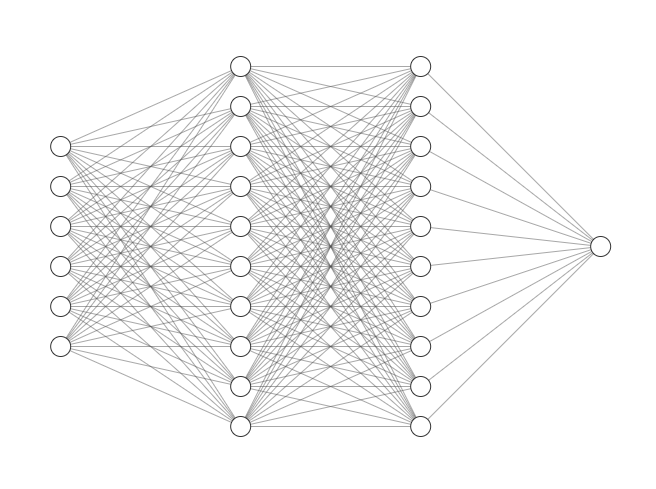
\includegraphics[width=0.9\textwidth]{figs/fcn.png}
% \caption{Przykładowa sieć w pełni połączona}
% \label{fig:fcn}
% \end{figure}

% Niech \(\bm{L}: \mathbb{R}^{n} \mapsto \mathbb{R}^{m}\) oznacza przekształcenie afiniczne postaci
% \[
% \bm{L}^\mu(\bm{x}; \bm{W}, \bm{b}) = \bm{b}^\mu + \sum_{\nu=1}^{n} \bm{W}^{\mu\nu}\bm{x}^\nu\,,
% \]
% gdzie \(\bm{W} \in \mathbb{R}^{m \times n}, \bm{b} \in \mathbb{R}^m\). Dodatkowo przez złożenie
% funkcji skalarnej \(a: \mathbb{R} \mapsto \mathbb{R}\) z funkcją \(\bm{L}\) będziemy rozumieć
% funkcję \(a \circ \bm{L} : \mathbb{R}^n \mapsto \mathbb{R}^m\)
% \[
% (a \circ \bm{L})^\mu (\bm{x}) = a\left(\bm{L}^\mu(\bm{x})\right) = a\left(\bm{b}^\mu + \sum_{\nu=1}^{n} \bm{W}^{\mu\nu}\bm{x}^\nu\right)\,.
% \]
% Sieć w pełni połączona złożona z \(k+2\) warstw o rozmiarach \(n_\text{in}, n_1, \ldots, n_k,
% n_\text{out}\) realizuje zatem przekształcenie \(\bm{\phi}: \mathbb{R}^{n_\text{in}} \mapsto
% \mathbb{R}^{n_\text{out}}\)
% \[
% \boxed
% {
% \bm{\phi}\left(\bm{x}; \left\{(\bm{W}_i, \bm{b}_i)\right\}_{i=1}^{k+1}\right) = \left( \bm{L}_{k+1} \circ a \circ \bm{L}_k \ldots a \circ \bm{L}_2 \circ a \circ \bm{L}_1 \right) (\bm{x}) \,,
% }
% \]
% gdzie \(\bm{L}_i : \mathbb{R}^{n_{i-1}} \mapsto \mathbb{R}^{n_i}\) (przy czym \(n_0 = n_\text{in}\)
% i \(n_{k+1} = n_\text{out}\))
% \[
% \boxed
% {
% \bm{L}_i^\mu \left(\bm{x}; \bm{W}_i, \bm{b}_i\right) = \bm{b}_i^\mu + \sum_{\nu=1}^{n_{i-1}} \bm{W}_i^{\mu\nu}\bm{x}^\nu\,,
% }
% \]
% \(\bm{W}_i \in \mathbb{R}^{n_i \times n_{i-1}}, \bm{b}_i \in \mathbb{R}^{n_i}\) (dla uproszczenia
% zapisu w miejscach, gdzie nie prowadzi to do niejasności będziemy oznaczać zbiór parametrów sieci
% \(\left\{(\bm{W}_i, \bm{b}_i)\right\}_{i=1}^{k+1}\) po prostu jako \(\bm{W}\)). Okazuje się, iż taka
% postać rodziny funkcji parametryzowanych przez wagi i obciążenia \(\bm{W}_i, \bm{b}_i\) potrafi
% aproksymować niemal dowolną funkcję (\textit{Universal Approximation Theorem}), zatem jest to niemal
% uniwersalny aproksymator, który możemy zastosować do wszelkich omawianych wcześniej zagadnień
% regresji i klasyfikacji. Zauważmy, iż już wcześniej rozwinęliśmy teorię w sposób dość ogólny
% wyprowadzając większość wyników dla pewnej dowolnej funkcji \(\bm{\phi}(\bm{x}; \bm{W})\) i jedynie
% na końcu znajdując dokładne rozwiązania dla prostego odwzorowania liniowego \(\bm{W}\bm{x}\) (na
% marginesie takie proste odwzorowanie odpowiada płytkiej sieci neuronowej o \(k=0\) warstwach
% ukrytych).

% W powyższej postaci sieć MLP przetwarza pojedynczo każdy wektor \(\bm{x}\) należący do zbioru danych
% \(\mc{X} = \{y_i(\bm{x}_i)\}_{i=1}^n\), a najbardziej kosztowną operacją jest mnożenie wektora przez
% macierz. Jest to jednak dość nieefektywne, gdyż na współczesnym sprzęcie mamy bardzo dobrze
% zoptymalizowane implementacje mnożenia macierzy przez siebie. Możemy jednak rozszerzyć odwzorowania
% \(\bm{L}\) i \(\bm{\phi}\) w taki sposób, aby sieć przetwarzała od razu cały \textit{batch} (tj.
% pewien podzbiór \(\mc{X} \supseteq \mc{B} = \{y_\beta(\bm{x}_\beta)\}\)) przykładów uczących
% reprezentowany przez macierz \(\bm{X}^{\beta \mu} = \bm{x}_\beta^\mu\) (stosujemy tutaj tzw.
% konwencję \textit{batch first} zgodnie z którą pierwszy indeks odpowiada kolejnym przykładom z
% batcha). Możemy zatem uogólnić postać przekształcenia \(\bm{\phi}\) jakie realizuje sieć do postaci
% \(\bm{\Phi}: \mathbb{R}^{n_\text{b} \times n_\text{in}} \mapsto \mathbb{R}^{n_\text{b} \times
% n_\text{out}}\), gdzie \(n_\text{b} = |\mc{B}|\)
% \[
% \bm{\Phi}\left(\bm{X}; \left\{(\bm{W}_i, \bm{b}_i)\right\}_{i=1}^{k+1}\right) = (\bm{L}_{k+1} \circ a \circ \bm{L}_k \ldots a \circ \bm{L}_2 \circ a \circ \bm{L}_1)(\bm{X})\,,
% \]
% gdzie \(\bm{L}_i: \mathbb{R}^{n_\text{b} \times n_{i-1}} \mapsto \mathbb{R}^{n_\text{b} \times n_i}\)
% \[
% \bm{L}_i^{\beta\mu}(\bm{X}; \bm{W}_i, \bm{b}_i) = \bm{b}_i^\mu + \sum_{\nu=1}^{n_{i-1}} \bm{W}_i^{\mu\nu} \bm{X}^{\beta\nu}\,,
% \]
% \(\bm{W}_i \in \mathbb{R}^{n_i \times n_{i-1}}, \bm{b}_i \in \mathbb{R}^{n_i}\). Przez złożenie
% funkcji skalarnej \(a: \mathbb{R} \mapsto \mathbb{R}\) z funkcją \(\bm{L}\) nadal rozumiemy
% \[
% (a \circ \bm{L})^{\beta\mu}(\bm{X}) = a(\bm{L}^{\beta\mu}(\bm{X}))\,.
% \]
% Widzimy zatem, iż tak naprawdę w takim sformułowaniu sieć przetwarza \(n_\text{b}\) przykładów
% równolegle zamiast przetwarzać je sekwencyjnie pojedynczo, co nie zmienia nic koncepcyjnie, a
% jedynie sprawia, iż sieć przetwarza dane bardziej efektywnie.

% \begin{quote}[\textit{Notes, Ch. 4} \cite{prince2023understanding}]
% \begin{itemize}
% \item \textbf{Deep learning}: It has long been understood that it is possible to build more complex
% functions by composing shallow neural networks or developing networks with more than one hidden
% layer. Indeed, the term “deep learning” was first used by Dechter (1986). However, interest was
% limited due to practical concerns; it was not possible to train such networks well. The modern era
% of deep learning was kick-started by startling improvements in image classification reported by
% [Alex] Krizhevsky et al. (2012) [AlexNet moment]. This sudden progress was arguably due to the
% confluence of four factors: larger training datasets, improved processing power for training, the
% use of the ReLU activation function, and the use of stochastic gradient descent.

% \item \textbf{Depth efficiency}: Several results show that there are functions that can be realized
% by deep networks but not by any shallow network whose capacity is bounded above exponentially. In
% other words, it would take an exponentially larger number of units in a shallow network to describe
% these functions accurately. This is known as the depth efficiency of neural networks.

% \item \textbf{Width efficiency}: Lu et al. (2017) investigate whether there are wide shallow
% networks (i.e., shallow networks with lots of hidden units) that cannot be realized by narrow
% networks whose depth is not substantially larger. They show that there exist classes of wide,
% shallow networks that can only be expressed by narrow networks with polynomial depth. This is known
% as the width efficiency of neural networks. This polynomial lower bound on width is less restrictive
% than the exponential lower bound on depth, suggesting that depth is more important. Vardi et al.
% (2022) subsequently showed that the price for making the width small is only a linear increase in
% the network depth for networks with ReLU activations.
% \end{itemize}
% \end{quote}


% \subsection{Funkcje kosztu}

% Tak jak zauważyliśmy wyżej wyprowadzoną wcześniej teorię można bezpośrednio zaaplikować dla
% przypadku sieci neuronowych. Wartości parametrów \(\bm{W}\) znajdujemy zatem w sposób analogiczny
% jak dla modeli klasycznych (tj. nie głębokich) minimalizując odpowiednią funkcję kosztu \(L(\mc{X};
% \bm{W})\) zależną od zbioru treningowego \(\mc{X}\) i parametrów sieci \(\bm{W}\), przy czym w
% czasie treningu \(\mc{X}\) jest ustalone, a dostosowujemy parametry \(\bm{W}\), natomiast w czasie
% inferencji wagi \(\bm{W}\) są ustalone (wytrenowane), a do sieci podajemy nowe przykłady. Wymienione
% wcześniej funkcje kosztu dla zagadnień regresji, klasyfikacji binarnej oraz wieloklasowej możemy
% zatem bezpośrednio wykorzystać uwzględniając jednak, iż odwzorowanie \(\bm{\phi}(\bm{x}; \bm{W})\)
% definiujące parametry określonego rozkładu prawdopodobieństwa jest teraz odpowiednią siecią
% neuronową. Nie ma tutaj więc żadnej zmiany jeśli chodzi o tworzenie modeli matematycznych
% rozważanych zagadnień w postaci odpowiednich parametrycznych modeli statystycznych, to co się
% zmienia to większa ekspresywność takich modeli dzięki wykorzystaniu sieci neuronowej jako
% uniwersalnego aproksymatora dla parametrów modelowanych rozkładów.

% Wcześniej wyprowadziliśmy funkcje kosztu (jako zanegowaną logarytmiczną funkcję wiarygodności) dla
% typowych zagadnień regresji i klasyfikacji -- odpowiednio błąd średniokwadratowy oraz entropię
% krzyżową i wieloklasową entropię krzyżową. Poniżej zamieszczamy tabelę zawierającą możliwe rozkłady
% prawdopodobieństwa, które można wykorzystać do skonstruowania funkcji kosztu dla mniej typowych
% zagadnień uczenia maszynowego.

% \begin{table}[ht]
% \centering
% \begin{tabular}{*5l}
% \toprule
% \textit{Domain} & \textit{Distribution} & \textit{Use} \\
% \midrule
% \(y \in \mathbb{R}\)            & univariate normal         & regression                \\ 
% \(y \in \mathbb{R}\)            & Laplace or t-distribution & robust regression         \\ 
% \(y \in \mathbb{R}\)            & mixture of gaussians      & multimodal regression     \\ 
% \(y \in \mathbb{R}_+\)          & exponential or gamma      & predicting magnitude      \\ 
% \(y \in [0;1]\)                 & beta                      & predicting proportion     \\ 
% \(\bm{y} \in \mathbb{R}^d\)     & multivariate normal       & multivariate regression   \\ 
% \(y \in (-\pi; +\pi]\)          & von Mises                 & predicting direction      \\ 
% \(y \in \{0,1\}\)               & Bernoulli                 & binary classification     \\ 
% \(y \in \{1,2,\ldots, K\}\)     & categorical               & multiclass classification \\ 
% \(y \in \{0,1,2,3,\ldots\}\)    & Poisson                   & predicting event counts   \\ 
% \(\bm{y} \in \mathrm{Perm}(n)\) & Plackett--Luce            & ranking                   \\ 
% \bottomrule
% \hline
% \end{tabular}
% \caption{\textit{Figure 5.11, Ch. 5, \cite{prince2023understanding}}}
% \end{table}

% % TODO: Actually derive loss functions for all the above

% \begin{quote}[\textit{Multiple outputs, Ch. 5,} \cite{prince2023understanding}]
% To make two or more prediction types simultaneously, we similarly assume the errors in each are
% independent. For example, to predict wind direction and strength, we might choose the von Mises
% distribution (defined on circular domains) for the direction and the exponential distribution
% (defined on positive real numbers) for the strength. The independence assumption implies that the
% joint likelihood of the two predictions is the product of individual likelihoods. These terms will
% become additive when we compute the negative log-likelihood.
% \end{quote}

% \begin{quote}[\textit{Notes, Ch. 5,} \cite{prince2023understanding}]
% \begin{itemize}
% \item \textbf{Class imbalance and focal loss}: Lin et al. (2017c) address data imbalance in
% classification problems. If the number of examples for some classes is much greater than for others,
% then the standard maximum likelihood loss does not work well; the model may concentrate on becoming
% more confident about well-classified examples from the dominant classes and classify less well-
% represented classes poorly. Lin et al. (2017c) introduce focal loss, which adds a single extra
% parameter that down-weights the effect of well-classified examples to improve performance.

% \item \textbf{Learning to rank}: Cao et al. (2007), Xia et al. (2008), and Chen et al. (2009) all
% used the Plackett--Luce model in loss functions for learning to rank data. This is the listwise
% approach to learning to rank as the model ingests an entire list of objects to be ranked at once.
% Alternative approaches are the pointwise approach, in which the model ingests a single object, and
% the pairwise approach, where the model ingests pairs of objects.

% \item \textbf{Non-probabilistic approaches}: It is not strictly necessary to adopt the probabilistic
% approach discussed in this chapter, but this has become the default in recent years; any loss
% function that aims to reduce the distance between the model output and the training outputs will
% suffice, and distance can be defined in any way that seems sensible. There are several well-known
% non-probabilistic machine learning models for classification, including support vector machines,
% which use hinge loss and AdaBoost, which uses exponential loss.
% \end{itemize}
% \end{quote}


% \subsection{Aspekty optymalizacyjne}

% Przedstawimy teraz algorytmy optymalizacji numerycznej najczęściej używane przy treningu głębokich
% sieci neuronowych. Jest oczywiste, iż nie jest możliwe znalezienie wartości wag sieci neuronowej
% minimalizujących funkcję kosztu \(L(\mc{X}; \bm{W})\) w sposób analityczny. Dodatkowo ze względu na
% ogromną liczbę parametrów współczesnych sieci (rzędu \(10^9\)) jakiekolwiek wyrafinowane algorytmy
% optymalizacji numerycznej (np. wykorzystujące drugie pochodne) również nie wchodzą w grę ze względu
% na zbyt duże wymagania pamięciowe. Biorąc pod uwagę wymienione ograniczenia skupimy się na prostych
% algorytmach optymalizacji pierwszego rzędu (z ang. \textit{first order methods}).

% Podstawowym algorytmem jest metoda spadku wzdłuż gradientu (z ang. \textit{gradient descent}).
% Polega ona na iteracyjnym aktualizowaniu wartości parametrów \(\bm{W}\) zgodnie z kierunkiem
% najszybszego spadku wyznaczonego przez zanegowany gradient funkcji kosztu \(-\pdv{L(\mc{X};
% \bm{W})}{\bm{W}}\). Wielkość kroków jakie wykonujemy w każdej iteracji jest zdeterminowana przez
% stałą \(\lambda > 0\) nazywaną \emph{stałą uczącą} (z ang. \textit{learning rate}). Tutaj należy
% dodać iż w implementacji wartość funkcji kosztu jest mnożona przez liczbę przykładów, w taki sposób,
% iż obliczamy tak naprawdę średni koszt na przykład, czyli \(L \gets \frac{1}{|\mc{X}|}L\). W
% przeciwnym wypadku wartość stałej uczącej należałoby dostosowywać do liczby przykładów w zbiorze.

% \begin{lstlisting}[language=Python, escapeinside={(*}{*)}]
% # Gradient descent
% # ----------------
% # Let (*$\mc{X}$*) be the whole training set.
% # Initialize heuristically parameters (*$\bm{W}$*) of the neural net.
% for epoch in range(max_epochs):
%     # Step 1. Compute derivatives of the loss function with
%     # respect to the parameters of neural net (*$\pdv{L(\mc{X}; \bm{W})}{\bm{W}}$*).

%     # Step 2. Update parameters of the neural net according to
%     (*$\bm{W} \gets \bm{W} - \lambda \pdv{L(\mc{X}; \bm{W})}{\bm{W}} $*)
%     # where (*$\lambda > 0$*) is a positive constant called 'learning rate'.
% \end{lstlisting}

% \begin{quote}[\textit{Gradient descent variants}, \cite{ruder2017overviewgradientdescentoptimization}]
% There are three variants of gradient descent, which differ in how much data we use to compute the
% gradient of the objective function. Depending on the amount of data, we make a trade-off between the
% accuracy of the parameter update and the time it takes to perform an update.
% \end{quote}

% Podstawowe modyfikacje powyższego algorytmu (zwanego również \textit{full-batch gradient descent})
% są związane z ograniczeniem zbioru treningowego dla którego obliczamy gradient. Podejście takie
% wynika z faktu, iż dla bardzo dużych zbiorów treningowych \(\mc{X}\) obliczane tensory mogą nie
% mieścić się w pamięci. Dodatkowo modyfikacja wprowadza losowość przy aktualizacji parametrów sieci,
% co pozwola na ucieczkę z lokalnych minimów funkcji kosztu. Aby rozwiązać ten problem dzielimy zbiór
% \(\mc{X}\) w każdej epoce na rozłączne \textit{batche} \(\mc{B}\) o tej samej wielkości
% \(n_\text{b}\) składające się z losowych przykładów ze zbioru \(\mc{X}\) (losowane bez zwracania i
% każdorazowo przy rozpoczęciu nowej epoki). Algorytm taki nazywamy \textit{batch gradient descent}
% lub \textit{mini-batch gradient descent}.

% \begin{lstlisting}[language=Python, escapeinside={(*}{*)}]
% # Mini-batch gradient descent
% # ---------------------------
% # Let (*$\mc{X}$*) be the whole training set.
% # Initialize heuristically parameters (*$\bm{W}$*) of the neural net.
% for epoch in range(max_epochs):
%     random_shuffle((*$\mc{X}$*))
%     for (*$\mc{B}$*) in get_batches((*$\mc{X}$*), batch_size):
%         # Step 1. Compute derivatives of the loss function with 
%         # respect to the parameters of neural net (*$\pdv{L(\mc{B}; \bm{W})}{\bm{W}}$*).

%         # Step 2. Update parameters of the neural net according to
%         (*$\bm{W} \gets \bm{W} - \lambda \pdv{L(\mc{B}; \bm{W})}{\bm{W}} $*)
%         # where (*$\lambda > 0$*) is a positive constant called 'learning rate'.
% \end{lstlisting}

% W szczególności gdy \(n_\text{b} = 1\), tj. każdy batch składa się z pojedynczego, losowo wybranego
% przykładu uczącego, to taki algorytm nazywamy \emph{stochastycznym spadkiem wzdłuż gradientu} (z
% ang. \textit{stochastic gradient descent, SGD}).

% \begin{quote}[\textit{Stochastic gradient descent}, \cite{ruder2017overviewgradientdescentoptimization}]
% Gradient descent performs redundant computations for large datasets, as it recomputes gradients for
% similar examples before each parameter update. SGD does away with this redundancy by performing one
% update at a time. It is therefore usually much faster and can also be used to learn online. SGD
% performs frequent updates with a high variance that cause the objective function to fluctuate
% heavily.

% While gradient descent converges to the minimum of the basin the parameters are placed in, SGD's
% fluctuation, on the one hand, enables it to jump to new and potentially better local minima. On the
% other hand, this ultimately complicates convergence to the exact minimum, as SGD will keep
% overshooting. However, it has been shown that when we slowly decrease the learning rate, SGD shows
% the same convergence behavior as batch gradient descent, almost certainly converging to a local or
% the global minimum for non-convex and convex optimization respectively.
% \end{quote}
 
% \begin{quote}[\textit{Mini-batch gradient descent}, \cite{ruder2017overviewgradientdescentoptimization}]
% Mini-batch gradient descent finally takes the best of both worlds and performs an update for every
% mini-batch of training examples. This way, it a) reduces the variance of the parameter updates,
% which can lead to more stable convergence; b) can make use of highly optimized matrix optimizations
% common to state-of-the-art deep learning libraries that make computing the gradient w.r.t. a
% mini-batch very efficient.

% Common mini-batch sizes range between 50 and 256, but can vary for different applications.
% Mini-batch gradient descent is typically the algorithm of choice when training a neural network and
% the term SGD usually is employed also when mini-batches are used.
% \end{quote}


% \subsubsection{Metoda pędu}

% W standardowym sformułowaniu SGD ma pewne problemy. Przede wszystkim dobór odpowiedniej wartości
% stałej uczącej do uzyskania dobrej zbieżności może być trudny. Dodatkowo istnieje poważny problem,
% który pojawia się przy minimalizacji silnie niewypukłych funkcji kosztu polegający na tym, iż
% algorytm utyka w lokalny minimum lub w punkcie siodłowym funkcji. Standardowy algorytm SGD nie
% posiada żadnych mechanizmów pozwalających na ucieczkę z tych punktów. Podstawowym ulepszeniem
% algorytmu SGD jest wprowadzenie tzw. pędu (z ang. \textit{momentum}) tj. członu postaci
% \[
% \bm{V}_t = \gamma \bm{V}_{t-1} - \lambda \pdv{L(\mc{B}; \bm{W})}{\bm{W}}\Big|_{\bm{W}}\,,\quad \bm{V}_0 = \bm{0}
% \]
% i aktualizację parametrów sieci zgodnie z
% \[
% \bm{W} \gets \bm{W} + \bm{V}_t\,,
% \]
% gdzie \(t\) jest numerem iteracji, a \(\gamma\) to tzw. \textit{momentum term}, którego wartość
% typowo przyjmuje się równą \(0.9\).

% \begin{quote}[\textit{Momentum}, \cite{ruder2017overviewgradientdescentoptimization}]
% Essentially, when using momentum, we push a ball down a hill. The ball accumulates momentum as it
% rolls downhill, becoming faster and faster on the way (until it reaches its terminal velocity, if
% there is air resistance, i.e. \(\gamma < 1\)). The same thing happens to our parameter updates: The
% momentum term increases for dimensions whose gradients point in the same directions and reduces
% updates for dimensions whose gradients change directions. As a result, we gain faster convergence
% and reduced oscillation.
% \end{quote}

% \subsubsection{Metoda Nesterova}

% \begin{quote}[\textit{Nesterov accelerated gradient}, \cite{ruder2017overviewgradientdescentoptimization}]
% However, a ball that rolls down a hill, blindly following the slope, is highly unsatisfactory. We
% would like to have a smarter ball, a ball that has a notion of where it is going so that it knows to
% slow down before the hill slopes up again.

% Nesterov accelerated gradient is a way to give our momentum term this kind of prescience. We know
% that we will use our momentum term \(\gamma \bm{V}_{t-1}\) to move the parameters \(\bm{W}\).
% Computing \(\bm{W} + \gamma \bm{V}_{t-1}\) thus gives us an approximation of the next position of
% the parameters (the gradient is missing for the full update), a rough idea where our parameters are
% going to be. We can now effectively look ahead by calculating the gradient not at our current
% parameters \(\bm{W}\) but at the approximate future position of our parameters:
% \[
% \begin{split}
% &\bm{V}_t = \gamma \bm{V}_{t-1} - \lambda \pdv{L(\mc{B}; \bm{W})}{\bm{W}}\Big|_{\bm{W} + \gamma \bm{V}_{t-1}}\,,\quad \bm{V}_0 = \bm{0}\,,\\
% &\bm{W} \gets \bm{W} + \bm{V}_t\,.
% \end{split}
% \]
% \end{quote}


% \subsubsection{Adam}

% \begin{quote}[\textit{Adam, Ch.6}, \cite{prince2023understanding}]
% Gradient descent with a fixed step size has the following undesirable property: it makes large
% adjustments to parameters associated with large gradients (where perhaps we should be more cautious)
% and small adjustments to parameters associated with small gradients (where perhaps we should explore
% further). When the gradient of the loss surface is much steeper in one direction than another, it is
% difficult to choose a learning rate that (i) makes good progress in both directions and (ii) is
% stable.

% A straightforward approach is to normalize the gradients so that we move a fixed distance (governed
% by the learning rate) in each direction.
% \[
% \begin{split}
% &\bm{G} = \pdv{L(\mc{B}; \bm{W})}{\bm{W}}\Big|_{\bm{W}}\,,\\
% &\bm{W} \gets \bm{W} - \lambda \frac{\bm{G}}{\sqrt{\bm{G}^2} + \epsilon}\,.
% \end{split}
% \]
% where the square root and division are both elementwise, \(\lambda\) is the learning rate, and
% \(\epsilon\) is a small constant that prevents division by zero when the gradient magnitude is zero.

% The result is that the algorithm moves a fixed distance \(\lambda\) along each coordinate, where the
% direction is determined by whichever way is downhill. This simple algorithm makes good progress in
% both directions but will not converge unless it happens to land exactly at the minimum. Instead, it
% will bounce back and forth around the minimum.

% \textit{Adaptive moment estimation}, or \textit{Adam}, takes this idea and adds momentum to both the
% estimate of the gradient and the squared gradient:
% \[
% \begin{split}
% &\bm{G} = \pdv{L(\mc{B}; \bm{W})}{\bm{W}}\Big|_{\bm{W}}\,,\\
% &\bm{M}_t = \beta_1 \bm{M}_{t-1} + (1 - \beta_1) \bm{G}  \,,\quad \bm{\tilde M}_t = \frac{\bm{M}_t}{1 - \beta_1^t}\,,\\
% &\bm{V}_t = \beta_2 \bm{V}_{t-1} + (1 - \beta_2) \bm{G}^2\,,\quad \bm{\tilde V}_t = \frac{\bm{V}_t}{1 - \beta_2^t}\,,\\
% &\bm{W} \gets \bm{W} - \lambda \frac{\bm{\tilde M}_t}{\sqrt{\bm{\tilde V}_t} + \epsilon}\,.
% \end{split}
% \]
% This algorithm can converge to the overall minimum and makes good progress in every direction in the
% parameter space.

% The choices of learning algorithm, batch size, learning rate schedule, and momentum coefficients are
% all considered hyperparameters of the training algorithm; these directly affect the final model
% performance but are distinct from the model parameters. Choosing these can be more art than science,
% and it is common to train many models with different hyperparameters and choose the best one. This
% is known as \textit{hyperparameter search}.
% \end{quote}

% \begin{quote}[\textit{Adam}, \cite{ruder2017overviewgradientdescentoptimization}]
% The authors propose default values of 0.9 for \(\beta_1\), 0.999 for \(\beta_2\), and \(10^{-8}\)
% for \(\epsilon\). They show empirically that Adam works well in practice and compares favorably to
% other adaptive learning-method algorithms.
% \end{quote}


% \subsection{Algorytm wstecznej propagacji błędu}

% W poprzednim paragrafie opisaliśmy podstawowe algorytmy wykorzystywane do minimalizacji funkcji
% kosztu, a co za tym idzie trenowania sieci neuronowych. Nie opisaliśmy jednak dwóch dość istotnych
% szczegółów: 1) jak właściwie obliczać gradient funkcji kosztu po parametrach sieci \(\pdv{L(\mc{B};
% \bm{W})}{\bm{W}}\); 2) w jaki sposób zainicjalizować wartości parametrów sieci. W tym paragrafie
% zajmujemy się pierwszym z wymienionych problemów, natomiast w następnym poruszamy kwestie
% regularyzacji oraz inicjalizacji głębokich sieci neuronowych.

% Sieć neuronowa (przetwarzająca od razu cały batch przykładów reprezentowany przez tablicę
% \(\bm{X}\)) jest tak naprawdę pewnym skierowanym, acyklicznym grafem (z ang. \textit{Directed
% Acyclic Graph, DAG}), zwanym \emph{grafem obliczeń}. Przykładowy graf obliczeń reprezentujący prostą
% sieć MLP z jedną warstwą ukrytą przedstawiono na rysunku \ref{fig:compgraph}.

% \begin{figure}[ht]
% \centering
% 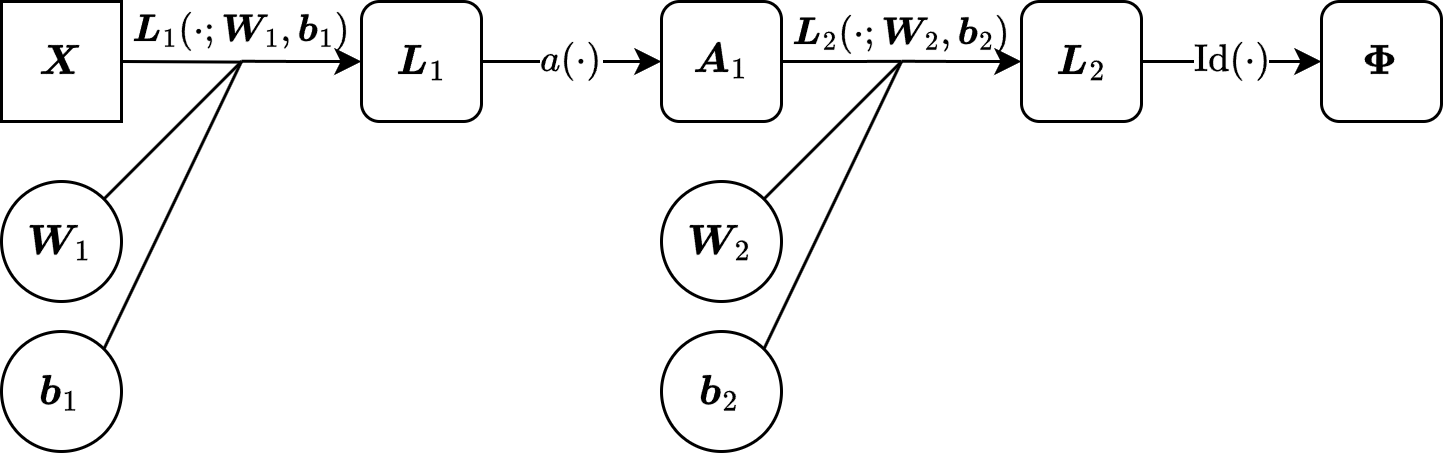
\includegraphics[width=0.85\textwidth]{figs/compgraph.png}
% \caption{Graf obliczeń reprezentujący prostą sieć MLP z jedną warstwą ukrytą}
% \label{fig:compgraph}
% \end{figure}

% Chcemy w sposób automatyczny z dokładnością do epsilon maszynowego obliczyć wartości pochodnych
% \(\pdv{L(\mc{X}; \bm{W})}{\bm{W}_i}\), \(\pdv{L(\mc{X}; \bm{W})}{\bm{b}_i}\). Zauważmy, iż zgodnie z
% regułą łańcuchową oznaczając
% \[
% \bm{\Delta}_i^{\mu_1\mu_2} = \pdv{L}{\bm{L}_i^{\mu_1\mu_2}}
% \]
% mamy
% \[
% \pdv{L}{\bm{W}_i^{\mu_1\mu_2}} = \sum_{\nu_1, \nu_2} \bm{\Delta}_i^{\nu_1\nu_2} \pdv{\bm{L}_i^{\nu_1\nu_2}}{\bm{W}_i^{\mu_1\mu_2}} = \sum_{\nu_1} \bm{\Delta}_i^{\nu_1\mu_1} \bm{A}_{i-1}^{\nu_1\mu_2}
% \]
% oraz
% \[
% \pdv{L}{\bm{b}_i^\mu} = \sum_\nu \bm{\Delta}_i^{\nu\mu}\,,
% \]
% gdzie oznaczamy \(\bm{A}_0 = \bm{X}\). Jednocześnie zauważmy, że
% \[
% \bm{\Delta}_i^{\mu_1\mu_2} = \sum_{\nu_1,\nu_2} \pdv{L}{\bm{A}_i^{\nu_1\nu_2}}\pdv{\bm{A}_i^{\nu_1\nu_2}}{\bm{L}_i^{\mu_1\mu_2}}
% \]
% oraz
% \[
% \pdv{L}{\bm{A}_i^{\nu_1\nu_2}} = \sum_{\gamma_1,\gamma_2} \pdv{L}{\bm{L}_{i+1}^{\gamma_1\gamma_2}}\pdv{\bm{L}_{i+1}^{\gamma_1\gamma_2}}{\bm{A}_i^{\nu_1\nu_2}} = \sum_{\gamma} \bm{\Delta}_{i+1}^{\nu_1\gamma}\bm{W}_{i+1}^{\gamma\nu_2}
% \]
% i
% \[
% \pdv{\bm{A}_i^{\nu_1\nu_2}}{\bm{L}_i^{\mu_1\mu_2}} = a'(\bm{L}_i^{\nu_1\nu_2}) \delta_{\mu_1\nu_1} \delta_{\mu_2\nu_2}\,,
% \]
% skąd
% \[
% \bm{\Delta}_i^{\mu_1\mu_2} = a'(\bm{L}_i^{\mu_1\mu_2}) \sum_\gamma \bm{\Delta}_{i+1}^{\mu_1\gamma}\bm{W}_{i+1}^{\gamma\mu_2}\,.
% \]
% Powyższe wyniki możemy zapisać w zwartych postaciach macierzowych
% \[
% \boxed
% {
% \pdv{L}{\bm{W}_i} = \bm{\Delta}_i^T \bm{A}_{i-1}\,,\quad \pdv{L}{\bm{b}_i} = \bm{\Delta}_i^T \bm{1}\,,\quad \bm{\Delta}_i = a'(\bm{L}_i) \odot \left(\bm{\Delta}_{i+1} \bm{W}_{i+1}\right)\,,
% }
% \]
% gdzie \(\bm{A}_0 = \bm{X}\) oraz \(\bm{\Delta}_{k+1} = \pdv{L}{\bm{\Phi}}\) (zauważmy tutaj, iż
% człon ten wyznaczyliśmy już powyżej dla typowych funkcji kosztu). Powyższy przykład to wyprowadzenie
% algorytmu wstecznej propagacji błędu dla typowej sieci w pełni połączonej (reprezentowanej przez
% graf obliczeń \ref{fig:compgraph} z powielonymi warstwami ukrytymi -- na rysunku przedstawiono sieć
% z jedną warstwą ukrytą). Algorytm obliczania pochodnych możemy zatem zapisać następująco.

% \begin{lstlisting}[language=Python, escapeinside={(*}{*)}]
% # Backpropagation through MLP
% # ---------------------------
% # Let k be the number of hidden layers of the MLP network.

% # Step 1. For given batch (*$\bm{X}$*) perform a forward pass 
% # by computing and memorizing arrays (*$\bm{L}_i, \bm{A}_i$*).

% (*$\bm{A}_0 = \bm{X}$*)

% for (*$i$*) in range(1, (*$k$*)+2):
%     # Compute and memorize
%     (*$\bm{L}_i = \bm{A}_{i-1} \bm{W}_i^T + \bm{b}_i$*)
%     (*$\bm{A}_i = a(\bm{L}_i)$*)

% # Compute loss (*$L(\mc{B}; \bm{W})$*) for the output (*$\bm{\Phi} = \bm{L}_{k+1}$*).

% # Step 2. Perform backpropagation

% # Initialize seed
% (*$\bm{\Delta}_{k+1} = \pdv{L(\mc{B}; \bm{W})}{\bm{\Phi}}$*)

% for (*$i$*) in range((*$k$*)+1, 0, -1):
%     # Compute gradients
%     (*$\pdv{L}{\bm{W}_i} = \bm{\Delta}_i^T \bm{A}_{i-1}\,,\quad \pdv{L}{\bm{b}_i} = \bm{\Delta}_i^T \bm{1}$*)
    
%     # Update seed
%     if (*$i$*) > 1:
%         (*$\bm{\Delta}_{i-1} = a'(\bm{L}_{i-1}) \odot \left(\bm{\Delta}_{i} \bm{W}_{i}\right)$*)

% \end{lstlisting}


% Powyższy algorytm jest specjalnie dostosowany do sieci w pełni połączonej. Możemy go jednak prosto
% uogólnić do dowolnego acyklicznego i skierowanego grafu obliczeń. Załóżmy, iż rozpatrujemy warstwę
% (wierzchołek w grafie zaznaczony zaokrąglonym kwadratem) \(\bm{F}\) zależną od pewnych parametrów
% \(\bm{W}\) (w szczególności warstwa może nie mieć żadnych parametrów). Dla dowolnej warstwy
% \(\bm{F}\) przez \({\bm{\bar{F}}}\) oznaczymy pochodną \({\bm{\bar{F}}} = \pdv{L}{\bm{F}}\). Wówczas z
% reguły łańcuchowej
% \[
% \pdv{L}{\bm{W}^{\mu_1..\mu_k}} = \sum_{\nu_1..\nu_l} {\bm{\bar{F}}}^{\nu_1..\nu_l} \pdv{\bm{F}^{\nu_1..\nu_l}}{\bm{W}^{\mu_1..\mu_k}}\,.
% \]
% Niech \(\mathrm{succ}(\bm{F})\) oznacza zbiór następników wierzchołka \(\bm{F}\), tj. warstw
% (wierzchołków w grafie zaznaczonych zaokrąglonym kwadratem) do których istnieje skierowana krawędź
% od warstwy \(\bm{F}\). Wówczas
% \[
% \bm{\bar{F}}^{\mu_1..\mu_k} = \pdv{L}{\bm{F}^{\mu_1..\mu_k}} = \sum_{\bm{S} \in \mathrm{succ}(\bm{F})} \sum_{\nu_1..\nu_l} \bm{\bar{S}}^{\nu_1..\nu_l} \pdv{\bm{S}^{\nu_1..\nu_l}}{\bm{F}^{\mu_1..\mu_k}}\,.
% \]
% Z powyższego zatem widzimy, iż możemy obliczać wielkości \(\bm{\bar{F}}\) w sposób iteracyjny
% przechodząc po warstwach w kolejności odwrotnej do ich porządku topologicznego (z ang.
% \textit{reversed topological order}) i zapamiętywać wartości \({\bm{\bar{F}}}\). Wówczas dla każdej
% warstwy pochodne \(\bm{\bar{S}}\) jej następników będą już obliczone i będziemy mogli obliczyć
% \({\bm{\bar{F}}}\). Naiwna implementacja powyższego schematu będzie wymagać bardzo dużo pamięci, gdyż
% dla każdej warstwy musimy przechowywać oprócz jej wartości \(\bm{F}\) również wartość pochodnej
% \({\bm{\bar{F}}}\). Zauważmy, iż w przypadku algorytmu wstecznej propagacji błędu dla sieci MLP nie
% musimy przechowywać pochodnych funkcji kosztu po wartościach warstw, a jedynie dynamicznie obliczamy
% i przekazujemy wstecz tzw. \emph{ziarno} (z ang. \textit{seed}) \(\bm{\Delta}\). Wynika to
% oczywiście z faktu, iż w przypadku sieci MLP warstwy tworzą skierowaną ścieżkę, czyli najprostszy
% DAG. W przypadku innych architektur sieci neuronowych tak nie musi być i wówczas każdą grupę warstw
% w obrębie której warstwy nie tworzą ścieżki należy oddzielnie przeanalizować pod kątem wykorzystania
% pamięci.

% \begin{quote}[\textit{Notes, Ch.7}, \cite{prince2023understanding}]
% \begin{itemize}
%     \item \textbf{Reducing memory requirements}: Training neural networks is memory intensive. We
%     must store both the model parameters and the pre-activations at the hidden units for every
%     member of the batch during the forward pass. Two methods that decrease memory requirements are
%     gradient checkpointing (Chen et al., 2016a) and micro-batching (Huang et al., 2019). In gradient
%     checkpointing, the activations are only stored every N layers during the forward pass. During
%     the backward pass, the intermediate missing activations are recalculated from the nearest check-
%     point. In this manner, we can drastically reduce the memory requirements at the computational
%     cost of performing the forward pass twice. In micro-batching, the batch is sub- divided into
%     smaller parts, and the gradient updates are aggregated from each sub-batch before being applied
%     to the network.
% \end{itemize}
% \end{quote}


% \subsection{Inicjalizacja}

% Jak zaznaczyliśmy wyżej ten paragraf poświęcimy zagadnieniu inicjalizacji parametrów sieci
% neuronowej, który jest wymaganym elementem opisanych algorytmów minimalizacji numerycznej.
% Najprostszym pomysłem inicjalizacji parametrów sieci neuronowych jest przyjęcie wartości 0 dla
% obciążeń \(\bm{b}_i\) i wylosowanie elementów macierzy wag \(\bm{W}_i\) niezależnie z rozkładu
% normalnego \(\mc{N}(0, \sigma^2)\). Powstaje pytanie jaka powinna być wartość wariancji
% \(\sigma^2\). Pewną odpowiedź na to pytanie sugeruje analiza wariancji elementów aktywacji w
% kolejnych warstwach
% \[
% \bm{L}_{i+1}^{\beta\mu} = \bm{b}_i^{\mu} + \sum_{\nu=1}^{n_{i-1}} \bm{A}_i^{\beta\nu} \bm{W}_i^{\mu\nu}\,.
% \]
% W przypadku inicjalizacji mamy \(\bm{b}_i^\mu = 0\) oraz \(\bm{W}_i^{\mu\nu} \sim \mc{N}(0,
% \sigma_{W_i}^2)\), zatem
% \[
% \mathbb{E}\left[\bm{L}_{i+1}^{\beta\mu}\right] = \sum_{\nu=1}^{n_{i-1}} \mathbb{E}\left[\bm{A}_i^{\beta\nu}\right] \cdot \mathbb{E}\left[\bm{W}_i^{\mu\nu}\right] = 0
% \]
% oraz
% \[
% \mathbb{V}\left[\bm{L}_{i+1}^{\beta\mu}\right] = \mathbb{E}\left[(\bm{L}_{i+1}^{\beta\mu})^2\right] - \mathbb{E}\left[\bm{L}_{i+1}^{\beta\mu}\right]^2 = \sum_{\nu=1}^{n_{i-1}} \mathbb{V}\left[\bm{A}_i^{\beta\nu}\right] \cdot \sigma_{W_i}^2\,.
% \]
% Zakładając, iż wariancje składowych aktywacji są równe \(\sigma_{A_i}^2\) oraz pochodzą z rozkładu
% symetrycznego wokół 0 mamy (dla funkcji aktywacji ReLU)
% \[
% \sigma_{A_{i+1}}^2 = \sum_{\nu=1}^{n_{i-1}} \frac{1}{2}\sigma_{W_i}^2 \sigma_{A_i}^2 = \frac{n_{i-1}}{2}\sigma_{W_i}^2 \sigma_{A_i}^2\,.
% \]
% Widzimy zatem, iż jeśli chcemy aby rozrzut wartości kolejnych aktywacji był podobny do poprzednich
% musi zachodzić
% \[
% \sigma_{W_i}^2 = \frac{2}{n_{i-1}}\,.
% \]
% Otrzymujemy zatem następującą heurystykę inicjalizacji
% \[
% \boxed
% {
% \bm{b}_i = \bm{0}\,,\quad \bm{W}_i^{\mu\nu} \sim \mc{N}\left(0, \frac{2}{n_{i-1}}\right)
% }
% \]
% zwaną \emph{inicjalizacją He}. Analogiczna analiza dla propagacji wstecznej, gdzie aktualizujemy
% \(\bm{\Delta}\) sugeruje z kolei przyjęcie
% \[
% \sigma_{W_i}^2 = \frac{2}{n_i}\,.
% \]
% Jeśli \(n_i \neq n_{i-1}\), tj. macierz \(\bm{W}_i\) nie jest kwadratowa, to jedną z możliwości jest
% przyjęcie średniej arytmetycznej \(\overline{n} = \frac{n_{i-1} + n_i}{2}\)
% \[
% \sigma_{W_i}^2 = \frac{2}{\overline{n}} = \frac{4}{n_{i-1} + n_i}\,.
% \]


% \subsection{Regularyzacja}

% Jak wspomnieliśmy we wstępie ważnym pojęciem w uczeniu maszynowym jest pojemność modeli. Model o
% dużej pojemności (czyli na przykład właśnie głęboka sieć neuronowa) może nastręczać poważnych
% problemów w trakcie uczenia przez zjawisko overfittingu. Model o dużej pojemności może perfekcyjne
% dopasować się do zbioru trenującego. Równocześnie może on zignorować strukturę, której wykrycie było
% w istocie celem uczenia. Przyczyną przeuczenia jest fakt, że każdy zbiór trenujący jest skończony:
% 1) jest skończoną próbą obserwacji z zagadnienia, które jest celem uczenia; 2) każdy zbiór trenujący
% opisuje więc problem uczenia w sposób niepełny; 3) model przeucza, gdy jego pojemność pozwala mu
% dopasować się do konkretnego zbioru trenującego w sposób uniemożliwiający uogólnianie na nowe
% przypadki. Problem ten jest tym istotniejszy, im mniejszy jest zbiór trenujący. Algorytmy i techniki
% służące do kontroli pojemności modelu nazywamy metodami regularyzacji (z ang. \textit{regularization
% methods}).

% \begin{itemize}
% \item \textbf{Weight decay}. Analogicznie jak w przypadku prostych modeli liniowych jedną z
% możliwości regularyzacji jest dodanie do funkcji kosztu \(L\) czynnika regularyzującego
% zawierającego odpowiednią sumę norm poszczególnych parametrów sieci
% \[
% L^*(\mc{X}; \bm{W}) = L(\mc{X}; \bm{W}) + \frac{\gamma_2}{2}\sum_{i=1}^{k+1}\sum_{\mu,\nu} (\bm{W}_{i}^{\mu\nu})^2+ \gamma_1\sum_{i=1}^{k+1}\sum_{\mu,\nu} |\bm{W}_i^{\mu\nu}|\,.
% \]
% Różnica między regularyzacją \(L^2\) i \(L^1\) jest taka, że norma \(L^2\) ,,zachęca” sieć do
% wybierania małych wag, ale nie dokładnie będących 0, natomiast \(L^1\) zmniejsza wagi, ale w
% szczególności prowadzi do wag wynoszących dokładnie 0. W związku z tym regularyzacja \(L^1\)
% przeprowadza selekcję cech - “wyłączy” te, które są mało ważne. Zwykle człony regularyzujące
% wprowadza się jedynie dla wag sieci, a nie dla obciążeń, skąd nazwa tej metody regularyzacji --
% \textit{weight decay}.

% \item \textbf{Metoda wczesnego stopu}. Najprostszym, a zarazem powszechnie stosowanym sposobem
% regularyzacji sieci neuronowych jest metoda wczesnego stopu (z ang. \textit{early stopping}). Polega
% ona na podziale zbioru \emph{treningowego} na mniejszy zbiór treningowy i tzw. \emph{zbiór
% walidacyjny}. W trakcie treningu monitorujemy błąd popełniany przez model na zbiorze walidacyjnym
% (ale do treningu używamy tylko zbioru treningowego). Przerywamy uczenie, gdy błąd na zbiorze
% walidacyjnym zaczyna rosnąć lub nie maleje przez wybraną liczbę epok. Dlaczego postęp uczenia
% monitorowany jest na zbiorze walidacyjnym (wydzielonym ze zbioru trenującego) a nie na zbiorze
% testowym? Monitorując przebieg uczenia na zbiorze testowym dobieralibyśmy parametry uczenia (np.
% ilość epok) tak, by dawały dobry wynik na zbiorze testowym. Wówczas wynik na zbiorze testowym mógłby
% być wyraźnie lepszy niż faktyczna skuteczność sieci w docelowym zastosowaniu. Nie możemy dobierać
% parametrów modelu wprost pod zbiór, na którym będziemy oceniać jego docelową skuteczność. Celem
% zbioru testowego jest ocena skuteczności modelu dla nowych obserwacji (niedostępnych w czasie
% uczenia).

% Takie podejście wymaga dość dużego zbioru danych, z których musimy wydzielić trzy zbiory: zbiór
% treningowy (na którym uczymy model), zbiór walidacyjny (na którym ewaluujemy model przy procedurze
% early stopingu) oraz zbiór testowy (na którym ewaluujemy model po treningu). Okres, przez który
% czekamy na uzyskanie lepszego wyniku, to cierpliwość (z ang. \textit{patience}). Im mniejsze, tym
% mocniejszy jest ten rodzaj regularyzacji, ale trzeba z tym uważać, bo łatwo jest przesadzić i zbyt
% szybko przerywać trening. Niektóre implementacje uwzględniają tzw. \textit{grace period}, czyli
% gwarantowaną minimalną liczbę epok, przez którą będziemy trenować sieć, niezależnie od wybranej
% cierpliwości.

% \item \textbf{Dropout}. Dobrym sposobem regularyzacji modeli uczenia maszynowego jest uśrednianie
% odpowiedzi wielu modeli popełniających różne błędy. Chcemy więc uczyć wiele modeli (rozwiązujących
% ten sam problem) w taki sposób, by modele te różniły się między sobą. Jest to tzw. uczenie zespołowe
% (z ang. \textit{ensemble learning}). Jak zapewnić, by wyuczone modele się między sobą różniły?
% Jednym ze sposobów budowy modelu zespołowego jest \emph{bagging} (od bootstrap aggregating)
% polegający na trenowaniu modeli na losowo wybranych (ze zwracaniem) podzbiorach zbioru treningowego,
% odpowiedzią modelu będzie średnia z odpowiedzi wszystkich wyuczonych w taki sposób modeli.
% Oczywiście w przypadku obliczeniowo kosztownych modeli jak sieci neuronowe zaimplementowanie takiego
% schematu wprost jest nieefektywne. Metodą, która efektywnie realizuje właśnie uczenie zespołowe na
% pojedynczej sieci neuronowej jest dropout. Polega on na tym, iż w procesie treningu ze z góry
% zadanym prawdopodobieństwem ,,wyłączamy'' wyjście neuronu (tj. dla każdej aktualizacji wartości
% parametrów sieci, w algorytmie wstecznej propagacji błędu mnożymy elementwise wyjście \(\bm{A}_i\)
% przez tensor \(\bm{D}_i\), którego każdy element może być równy \(0\) z prawdopodobieństwem \(p_i\)
% lub \(1\) z prawdopodobieństwem \(1-p_i\)). Mechanizmu dropout używamy tylko w procesie treningu. W
% przypadku inferencji wyjście warstwy \(\bm{A}_i\) jest z kolei mnożone przez \(1 - p_i\), czyli
% prawdopodobieństwo pozostania neuronu w sieci (\emph{weight scaling inference rule}). Typowo usuwa
% się dość sporo neuronów w warstwach ukrytych, np. 50\%. Dzięki dropoutowi można używać dość dużych
% stałych uczących oraz współczynników pędu, a także trenować znacznie większe i głębsze sieci.
% Okazuje się, iż w praktyce takie duże, mocno trenowane sieci z regularyzacją uczą się lepiej niż
% mniejsze, które by tej regularyzacji nie potrzebowały. Jeśli sieć nie przeucza na zbiorze trenującym
% to najpewniej lepsze wyniki uzyskamy ucząc większą sieć (która normalnie mogłaby przeuczyć) i
% stosując dropout. Obecnie dropout jest powszechnie stosowanym sposobem regularyzacji warstw w pełni
% połączonych (np. ostatnich warstw w niektórych sieciach konwolucyjnych).

% \item \textbf{Transfer learning}. 
% \begin{quote}[\textit{Transfer learning and multi-task learning, Ch.9},
% \cite{prince2023understanding}] When training data are limited, other datasets can be exploited to
% improve performance. In transfer learning, the network is pre-trained to perform a related secondary
% task for which data are more plentiful. The resulting model is then adapted to the original task.
% This is typically done by removing the last layer and adding one or more layers that produce a
% suitable output. The main model may be fixed, and the new layers trained for the original task, or
% we may fine-tune the entire model. The principle is that the network will build a good internal
% representation of the data from the secondary task, which can subsequently be exploited for the
% original task. Equivalently, transfer learning can be viewed as initializing most of the parameters
% of the final network in a sensible part of the space that is likely to produce a good solution.
% \end{quote}

% \item \textbf{Augmentation}. Metoda data augmentation polega na dodaniu do zbioru treningowego
% replik przykładów z tego zbioru poddanych pewnym transformacjom względem których oczekujemy, iż
% odpowiedzi sieci będą niezmienione.
% \end{itemize}


% \subsection{Hiperparametry}

% \subsubsection{Dobór hiperparametrów}

% \begin{quote}[\textit{Choosing hyperparameters, Ch.8}, \cite{prince2023understanding}]
%     For a deep network, the model capacity depends on the numbers of hidden layers and hidden units per
%     layer as well as other aspects of architecture that we have yet to introduce. Furthermore, the
%     choice of learning algorithm and any associated parameters (learning rate, etc.) also affects the
%     test performance. These elements are collectively termed hyperparameters. The process of finding the
%     best hyperparameters is termed hyperparameter search or (when focused on network structure) neural
%     architecture search.
    
%     Hyperparameters are typically chosen empirically; we train many models with different
%     hyperparameters on the same training set, measure their performance, and retain the best model.
%     However, we do not measure their performance on the test set; this would admit the possibility that
%     these hyperparameters just happen to work well for the test set but don't generalize to further
%     data. Instead, we introduce a third dataset known as a validation set. For every choice of
%     hyperparameters, we train the associated model using the training set and evaluate performance on
%     the validation set. Finally, we select the model that worked best on the validation set and measure
%     its performance on the test set. In principle, this should give a reasonable estimate of the true
%     performance. 
    
%     The hyperparameter space is generally smaller than the parameter space but still too
%     large to try every combination exhaustively. Unfortunately, many hyperparameters are discrete (e.g.,
%     the number of hidden layers), and others may be conditional on one another (e.g., we only need to
%     specify the number of hidden units in the tenth hidden layer if there are ten or more layers).
%     Hence, we cannot rely on gradient descent methods as we did for learning the model parameters.
%     Hyperparameter optimization algorithms intelligently sample the space of hyperparameters, contingent
%     on previous results. This procedure is computationally expensive since we must train an entire model
%     and measure the validation performance for each combination of hyperparameters.    
% \end{quote}


% \subsubsection{Zjawisko double descent}

% Zjawisko double descent polega na nieoczekiwanym zachowaniu wartości błędów popełnianych przez model
% uczenia maszynowego przy zwiększaniu liczby jego parametrów. Zgodnie z bias-variance tradeoff
% oczekiwalibyśmy bowiem iż w miarę zwiększania liczby parametrów będziemy coraz bardziej przeuczać
% model (dopasowywać go wprost do danych treningowych), a przez to zmniejszać jego zdolność
% generalizacji, co przekładałoby się na gorszy wynik na zbiorze testowym. Okazuje się jednak, iż
% krzywa błędu na zbiorze testowym w zależności od liczby parametrów początkowo spada, następnie
% (zgodnie z oczekiwaniami) gdy liczba parametrów jest rzędu liczności zbioru treningowego błąd
% rośnie, ale (co niespodziewane) gdy liczba parametrów jest znacznie większa od liczności zbioru
% treningowego, błąd testowy znowu spada.

% \begin{quote}[\textit{Double descent, Ch.8}, \cite{prince2023understanding}]
% This phenomenon is known as double descent. For some datasets like MNIST, it is present with the
% original data. For others, like MNIST-1D and CIFAR-100, it emerges or becomes more prominent when we
% add noise to the labels. The first part of the curve is referred to as the \emph{classical} or
% \emph{under-parameterized regime}, and the second part as the \emph{modern} or
% \emph{over-parameterized regime}. The central part where the error increases is termed the critical
% regime.
% \end{quote}

% \begin{figure}[ht]
% \centering
% 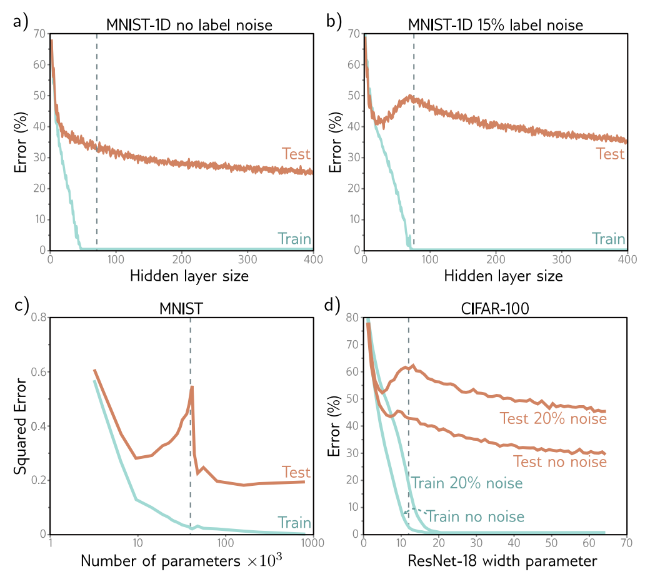
\includegraphics[width=0.8\textwidth]{figs/double_descent.png}
% \caption{Przykładowa krzywa wartości błędu na zbiorze testowym w zależności od liczby parametrów modelu wykazująca efekt double descent}
% \label{fig:double-descent}
% \end{figure}

% \begin{quote}[\textit{Double descent, Ch. 8}, \cite{prince2023understanding}]
% To understand why performance continues to improve as we add more parameters, note that once the
% model has enough capacity to drive the training loss to near zero, the model fits the training data
% almost perfectly. This implies that further capacity cannot help the model fit the training data any
% better; any change must occur between the training points. The tendency of a model to prioritize one
% solution over another as it extrapolates between data points is known as its inductive bias.

% The putative explanation for double descent is that as we add capacity to the model, it interpolates
% between the nearest data points increasingly smoothly. In the absence of information about what
% happens between the training points, assuming smoothness is sensible and will probably generalize
% reasonably to new data.

% However, this does not explain why over-parameterized models should produce smooth functions. The
% answer to this question is uncertain, but there are two likely possibilities. First, the network
% initialization may encourage smoothness, and the model never departs from the sub-domain of smooth
% function during the training process. Second, the training algorithm may somehow “prefer” to
% converge to smooth functions. Any factor that biases a solution toward a subset of equivalent
% solutions is known as a regularizer, so one possibility is that the training algorithm acts as an
% implicit regularizer.
% \end{quote}


% \subsection{Sieci konwolucyjne}

% Przechodzimy teraz do opisu konkretnych architektur sieci neuronowych innych niż sieci w pełni
% połączone. Pierwszą architekturą, którą opiszemy będą sieci konwolucyjne. Sieci konwolucyjne (z ang.
% \emph{Convolutional Neural Networks, CNN}) to architektura sieci neuronowych przystosowana do
% przetwarzania danych posiadających pewne zależności przestrzenne, przez co rozumiemy, iż jeśli
% \(\bm{X}^{i...j}\) jest tensorem wejściowym to zależności występują między wartościami sąsiednimi.
% Przykładem takich danych są oczywiście obrazy. Przetwarzanie takich danych przez sieć MLP byłoby
% niezwykle nieefektywne, gdyż połączenia każdy z każdym oznaczałyby iż przykładowo dla obrazu w skali
% szarości o rozdzielczości \(512 \times 512\) mielibyśmy rzędu \(10^9\) parametrów dla jednej warstwy
% ukrytej. Dodatkowo sieć MLP szukałaby powiązań między odległymi pikselami, pomiędzy którymi takich
% zależności nie ma. Sieć CNN robi to znacznie efektywniej wykorzystując warstwy konwolucyjne. 

% Załóżmy, iż przetwarzamy cały batch obrazów rozmiaru, z których każdy jest reprezentowany przez
% 3-tensor (tj. tensor o 3 osiach) o wymiarach \((h, w, c)\), gdzie \(h\) to wysokość, \(w\) to
% szerokość, a \(c\) to liczba kanałów (przykładowo równa 3 dla zdjęć w kolorze). Cały batch jest
% zatem reprezentowany przez tensor \(\bm{X} \in \mathbb{R}^{b \times h \times w \times c }\), gdzie
% \(b\) to liczba przykładów w batchu. Warstwa konwolucyjna (z ang. \emph{Convolutional Layer})
% realizuje następujące przekształcenie (zakładamy, iż indeksy zaczynają się od 0)
% \[
% \boxed
% {
% \begin{split} 
% &\bm{C}: \mathbb{R}^{b \times h_\text{in} \times w_\text{in} \times c_\text{in}} \mapsto \mathbb{R}^{b \times h_\text{out} \times w_\text{out} \times c_\text{out}}\\
% &\bm{C}^{ijkl}(\bm{X}) = \bm{b}^{l} + \sum_{p = 0}^{h_f-1} \sum_{q = 0}^{w_f-1} \sum_{r = 0}^{c_\text{in}-1} \bm{W}^{lpqr} \bm{X}^{i, s_h j + d_h p, s_w k + d_w q, r}
% \end{split}
% }
% \]
% Tensor \(\bm{W} \in \mathbb{R}^{c_\text{out}\times h_f \times w_f \times c_\text{in}}\) nazywamy
% \emph{mapą konwolucyjną}, a tensor \(\bm{W}^{l,:,:,:}\) dla ustalonego \(l\) -- \emph{filtrem
% konwolucyjnym}. Formalnie opisane przekształcenie nie jest konwolucją, tylko \emph{korelacją
% skrośną}, ale dla nas rozróżnienie między obiema operacjami nie jest istotne. Wielkości \(s_h, s_w,
% d_h, d_w\) są ustalonymi stałymi dla danej warstwy konwolucyjnej zwanymi odpowiednio \emph{stride} i
% \emph{dilation}.

% Warstwę konwolucyjną charakteryzuje szereg parametrów:
% \begin{itemize}
% \item liczba kanałów wejściowych \(c_\text{in}\)
% \item liczba kanałów wyjściowych równą liczbie filtrów \(c_\text{out}\)
% \item wysokość i szerokość tzw. \textit{pola odbiorczego} (lub filtra) \(h_f, w_f\)
% \item \textit{stride} \(s\), zwykle jednakowy dla wymiaru góra-dół i lewo-prawo chociaż w ogólności
% możemy przyjąć różne wartości \(s_h, s_w\). Parametr ten określa o ile przesuwamy pole odbiorcze w
% każdym kroku.
% \item \textit{dilation rate} \(d\), ponownie zwykle jednakowy dla obu wymiarów chociaż w ogólności
% \end{itemize}

% Podanie powyższych parametrów warstwy konwolucyjnej jednoznacznie wyznacza wymiary obrazu tensora po
% konwolucji. Istotnie zauważmy, iż musi zachodzić
% \[
% s_h(h_\text{out} - 1) + d_h (h_f - 1) \leq h_\text{in} - 1\,,\quad s_w(w_\text{out} - 1) + d_w (w_f - 1) \leq w_\text{in} - 1
% \]
% skąd
% \[
% h_\text{out} = \left\lfloor \frac{h_\text{in} - 1 - d_h (h_f - 1)}{s_h} + 1 \right\rfloor\,,\quad w_\text{out} = \left\lfloor \frac{w_\text{in} - 1 - d_w (w_f - 1)}{s_w} + 1 \right\rfloor\,.
% \]
% Do algorytmu wstecznej propagacji błędu potrzebujemy oczywiście znać jeszcze pochodne
% \(\pdv{\bm{C}}{\bm{X}}\) oraz \(\pdv{\bm{C}}{\bm{W}}\), które można w łatwy sposób wyznaczyć
% \[
% \begin{split}
% \pdv{\bm{C}^{ijkl}}{\bm{X}^{abcd}} &= \sum_{p = 0}^{h_f-1} \sum_{q = 0}^{w_f-1} \sum_{r = 0}^{c_\text{in}-1} \bm{W}^{lpqr} \cdot \delta_{i,a} \cdot \delta_{s_h j + d_h p, b} \cdot \delta_{s_w k + d_w q, c} \cdot \delta_{r, d}\\
% &= \bm{W}^{l, b/d_h - s_h j/d_h, c/d_w - s_w k/d_w, d} \delta_{i,a}\\
% \pdv{\bm{C}^{ijkl}}{\bm{W}^{abcd}} &= \sum_{p = 0}^{h_f-1} \sum_{q = 0}^{w_f-1} \sum_{r = 0}^{c_\text{in}-1} \bm{X}^{i, s_h j + d_h p, s_w k + d_w q, r} \delta_{l,a} \delta_{p,b} \delta_{q,c} \delta_{r,d}\\
% &= \bm{X}^{i, s_h j + d_h b, s_w k + d_w c, d} \delta_{l,a}
% \end{split}
% \]

% Opiszmy jeszcze pokrótce jak implementowane są warstwy konwolucyjne. Zwykle nie implementuje się ich
% bezpośrednio z definicji tylko korzysta z tzw. transformacji \emph{im2col}, która zamienia 3-tensor
% (np. zdjęcie) w macierz, której kolumny to spłaszczone pola odbiorcze po których będzie przechodził
% filtr, natomiast pojedynczy filtr jest przekształcany do wektora wierszowego. Poszczególne filtry z
% mapy konwolucyjnej są potem łączone w macierz i wykonujemy zwykłe mnożenie macierzowe między
% macierzą filtrów oraz macierzą im2col. Takie podejście pozwala wykorzystać bardzo wydajne procedury
% do mnożenia macierzy. Poniżej na rysunku \ref{fig:conv} przedstawiono prostą wizualizację opisanej
% procedury dla przypadku \(c_\text{in} = 3\), \(c_\text{out} = 4\), \(h_\text{in} = w_\text{in} =
% 6\), \(h_f = w_f = s_h = s_w = 2\), \(d_h = d_w = 1\). Dla ułatwienia wizualizacji przyjęliśmy \(d_h
% = d_w = 1\) oraz \(s_h = h_f\) i \(s_w = w_f\), w przeciwnym wypadku pola odbiorcze na siebie
% zachodzą i/lub sąsiednie komórki w polu odbiorczym są od siebie oddalone o \(d > 1\). Zasada
% tworzenia macierzy za pomocą im2col jest jednak wówczas identyczna, tj. poszczególne kolumny w
% macierzy odpowiadają polom odbiorczym w kolejnych kanałach.

% \begin{figure}[ht]
% \centering
% 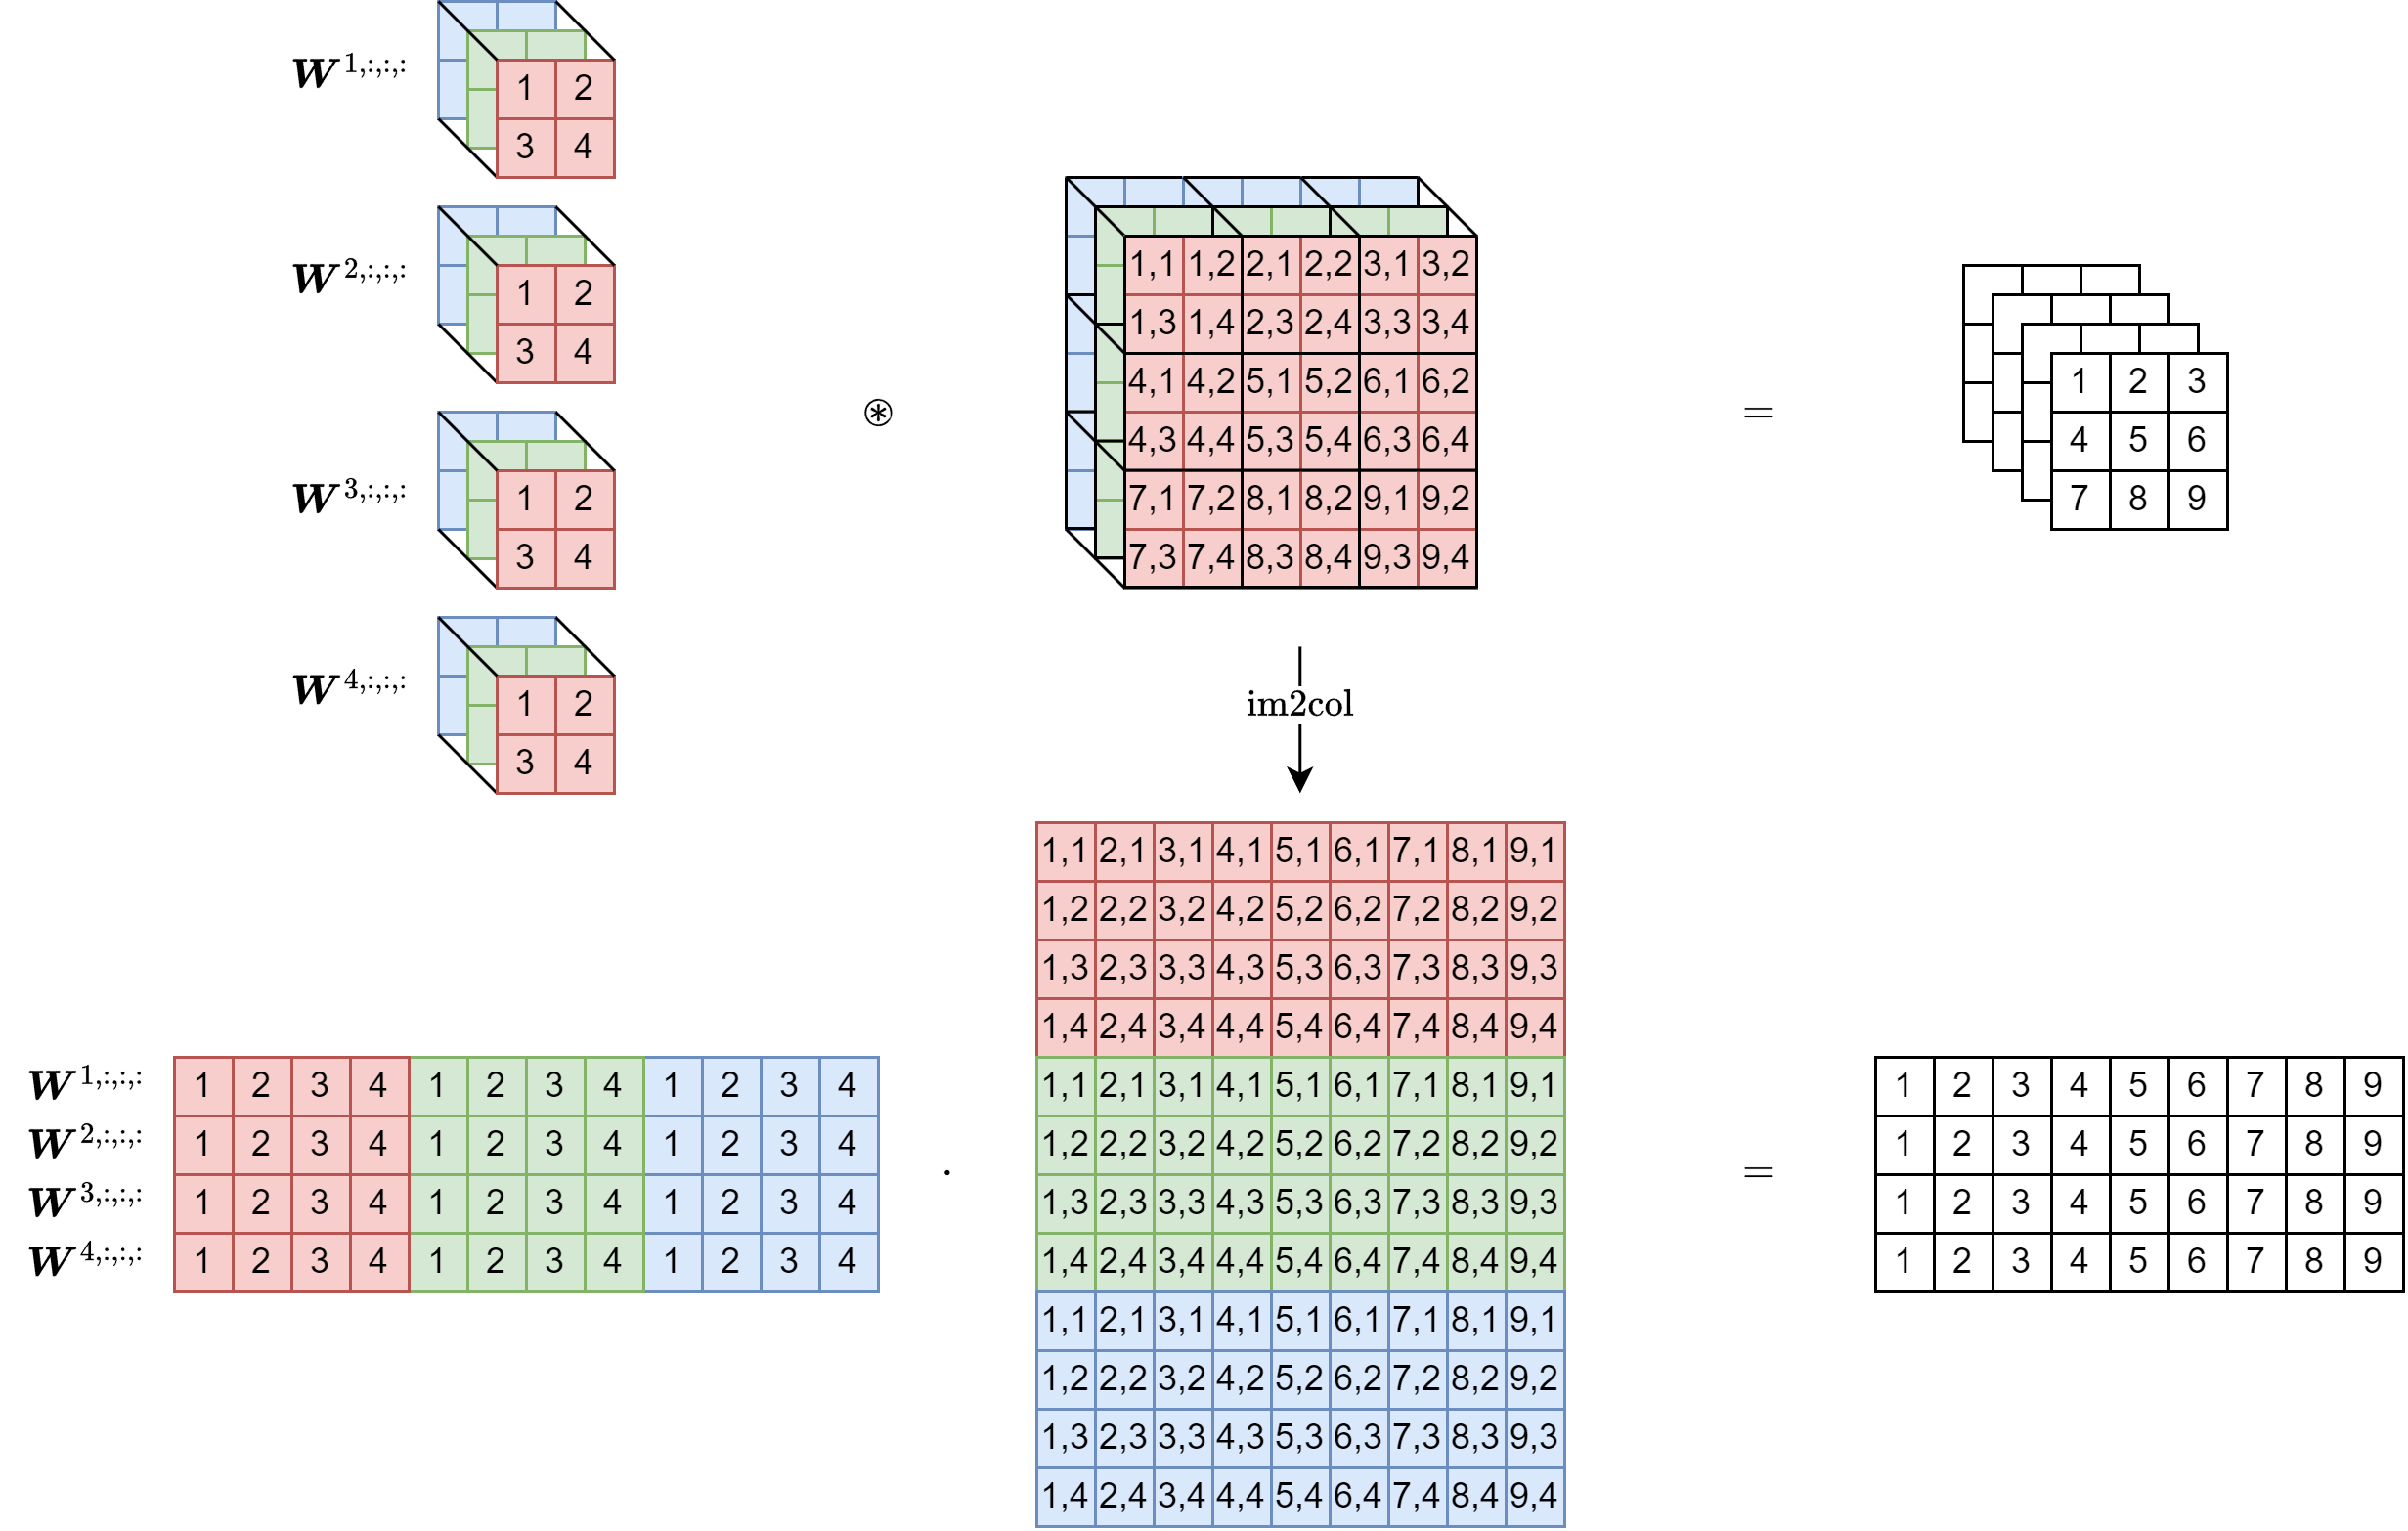
\includegraphics[width=0.85\textwidth]{figs/conv.png}
% \caption{Wizualizacja implementacji konwolucji jako mnożenia macierzy}
% \label{fig:conv}
% \end{figure}

% Drugim rodzajem warstw typowo wykorzystywanym w sieciach CNN są tzw. warstwy poolingowe
% (zbierające). Są to warstwy bezparametrowe, które z pola odbiorczego wyciągają pojedynczą liczbę.
% Operują na każdym kanale niezależnie, przez co nie zmieniają wymiaru głębi, ale pozwalają zredukować
% wymiar przestrzenny. Najczęściej stosowane są warstwy typu max pooling wyciągające wartość
% największą lub average pooling, które biorą średnią z wartości w polu odbiorczym.


% \subsubsection{Ekwiwariancja i inwarianja}

% Żeby zobrazować różnicę między ekwiwariancją a inwariancją, weźmy zadanie wykrywania twarzy. Chcemy
% wykryć wszystkie twarze, niezależnie od tego, gdzie się znajdują. W związku z tym filtry wykrywające
% oczy, usta, nos etc. muszą aktywować się wielokrotnie i w różnych miejscach obrazu - chcemy
% ekwiwariancji, to daje nam warstwa konwolucyjna. Nie obchodzi nas jednak, gdzie dokładnie co do
% piksela względem siebie są te elementy twarzy, tylko żeby były mniej więcej w podobnych pozycjach -
% oczy po przeciwnych stronach nosa, nos poniżej oczu. Chcemy więc inwariancji ze względu na takie
% niewielkie translacje. Uwaga sieci konwolucyjne nie są ekwiwariantne/inwariantne ze względu na
% rotację, przybliżenie, odbicie, zmianę oświetlenia etc. Z tego powodu przeprowadza się wzbogacanie/
% augmentację zbioru uczącego, czyli dodanie sztucznych przykładów stworzonych przez transformacje
% oryginalnego zbioru treningowego. Dzięki temu sieć ma okazję zobaczyć takie modyfikacje i się ich
% nauczyć.


% \subsubsection{Interpretowalność}

% Jedną ze słabych stron sieci konwolucyjnych (i sieci neuronowych w ogóle) jest niska
% interpretowalność. Wiemy, że sieć uczy się cech pozwalających skutecznie rozpoznawać obrazy, ale
% jakie w istocie są to cechy? Stosunkowo prosty trik pozwala w ciekawy sposób zobrazować
% interpretację wejściowego obrazu w poszczególnych warstwach CNN. Podstawowa idea polega tu na takiej
% modyfikacji wejściowego obrazu, aby wzmocnić jego reprezentację w wybranej warstwie konwolucyjnej.
% Jeżeli więc aktywacje w obrazowanej warstwie wynoszą \(\bm{A}\), to wykonywana jest wsteczna
% propagacja błędu (począwszy od obrazowanej warstwy) dla funkcji kosztu proporcjonalnej do
% \(-\norm{\bm{A}}_\text{Frobenius}\). Gradient propagowany jest do wejściowego obrazu włącznie. W
% efekcie wejściowy obraz jest modyfikowany w taki sposób, by w obrazowanej warstwie wzrosła
% amplituda.


% \subsubsection{Połączenia rezydualne}

% W przypadku klasycznej (sekwencyjnej) architektury CNN przy pewnej liczbie warstw ukrytych
% skuteczność ulega wysyceniu. Dalsze zwiększanie głębokości sieci prowadzi do zjawiska degradacji.
% Czy można zapobiec zjawisku degradacji w głębokiej sieci konwolucyjnej? Tak! Jedną z architektur, w
% której zjawisko degradacji nie występuje są sieci rezydualne (ResNety). Architektura sieci
% rezydualnych wywodzi się z heurystycznej/eksperymentalnej obserwacji, wedle której modelowanie
% nieliniowego przekształcenia \(\bm{f}(\bm{x})\) jest nierzadko trudniejsze, niż modelowanie
% przekształcenia rezydualnego \(\bm{f}(\bm{x}) - \bm{x}\). Podstawową jednostką funkcjonalną w
% sieciach ResNet są więc bloki rezydualne, które propagują aktywacje dwoma ścieżkami: poprzez
% sekwencję konwolucji i funkcji aktywacji oraz drugą ścieżką poprzez funkcję identycznościową.
% Sygnały na końcu tych ścieżek są sumowane.

% % ========================================================.
% % TODO::                                                  |
% % ========================================================|
% % ////////////////////////////////////////////////////////|
% % --------------------------------------------------------|
% % Classical ML                                            |
% % --------------------------------------------------------|
% % * CART, boosting, bagging                               |
% % * PCA (SVD / eigenvalue decomposition)                  |
% % --------------------------------------------------------|
% % Deep Learning                                           |
% % --------------------------------------------------------|
% % * Attention, Transformers, LLMs                         |
% % * Universal Transformer / NN                            |
% % * GANs                                                  |
% % * DDPMs                                                 |
% % * Autoencoders                                          |
% % * Boltzmann machines                                    |
% % ========================================================|
% % ////////////////////////////////////////////////////////|
% % ========================================================.

% \bibliographystyle{plain}
% \bibliography{refs} % Entries are in the refs.bib file

